\chapter{Unparse Algorithmus}

In diesem Kapitel wird der Algorithmus zum Unparsen von Variation-Trees und Methode Variation-Diffs umzuparsen vorgestellt. Wir beschreiben den theoretischen Hintergrund, welche Bedingungen erfühlt werden müssen, damit der Algorithmus korrekt funktioniert und die Arbeitsweise des Algorithmus.\\

Wir beschäftigen uns mit der Definition von Variation-Tree und Variation-Diff, nehmen neue Definitionen für Variation-Tree und Variation-Diff aus anderer Arbeit und erweitern diese. Es werden auf Bedingungen aufgestellt, ohne die der Algorithmus nicht korrekt funktionieren kann. Der von uns entwickelte Algorithmus basiert auf der Tiefensuche und kann nur für das unparsen von Variation-Trees verwendet werden. Für das Unparsen von Variation-Diffs reduzieren wir das Problem. Indem wir statt Variation-Diff zu unparsen, den Variation-Diff projizieren, dann zwei Variation-Trees unparsen und schließlich ein Diff über das Ergebnis bilden.\\

Wir fangen an mit Definitionen von Variation-Tree und Variation-Diff in Kapitel 3.1. Danach im Kapitel 3.2 sehen wir den Parser, welcher Variation-Trees und Variation-Diffs erstellt. Im Kapitel 3.3 werden die, während des Parsens, verlorengehende Informationen bestimmt und Möglichkeiten vorgestellt diese zurückzubekommen. Aufbauend auf den vorherigen wird im Kapitel 3.4 unser Algorithmus zum Unparsen von Variation-Trees vorgestellt. Schlussendlich wird im Kapitel 3.5 eine Laufzeitanalyse des Algorithmus durchgeführt.




\section{Variation-Tree und Variation-Diff}

Um verstehen zu können, wie wir Variation-Trees und -Diffs unparsen können, müssen wir uns mit den Einschränkungen und Möglichkeiten des Parsers vertraut machen.\\


Um Variation-Trees und Variation-Diffs kennenzulernen, betrachten wir zunächst die ursprüngliche Definition der Datenstrukturen~\cite{BTS+:ESECFSE22}.
\begin{definition}
	Ein \textsc{Variation-Tree}  $(V,E,r,\tau,l)$ ist ein Baum mit Knoten $V$, Kanten $E \subseteq V \times V$ und Wurzelknoten $r \in V$. Jede Kante $(x,y) \in E$ verbindet einen Kinderknoten $x$ mit seinem Elternknoten $y$, bezeichnet mit $p(x) = y$. Der Knotentyp $\tau(v) \in $ \{\textsc{artifact,mapping,else}\} identifiziert einen Knoten $v \in V$ entweder als Vertreter eines Implementierungsartefakts, einer Feature-Annotation oder eines else-Zweigs. Das Label $l(v)$ ist eine aussagenlogische Formel, wenn $\tau(v) =$ \textsc{mapping}, ein Verweis auf ein Implementierungsartefakt, wenn $\tau(v) = $ \textsc{artifact}, oder leer, wenn $\tau(v) =$ \textsc{else} ist. Der Wurzelknoten $r$ hat den Typ $\tau(r) =$ \textsc{mapping} und das Label $l(r) = $ \textsc{true}. Ein Knoten $e$ von Typ $\tau(e) =$ \textsc{else} kann nur unterhalb eines Nichtwurzelknotens $v$ mit dem Typ $\tau(v) =$ \textsc{mapping} platziert werden, dabei hat ein Knoten $w$ von Typ $\tau(w) =$ \textsc{mapping} höchstens einen Knoten $u$ von dem Typ $\tau(u) =$ \textsc{else}.
\end{definition}
\begin{definition}
	Ein \textsc{Variation-Diff} ist ein gerichteter, zusammenhängender, azyklischer Graph $D=(V,E,r,\tau,l,\Delta) $, welcher einen Wurzelknoten hat, mit Knoten $V$, Kanten $E \subseteq V \times V$, Wurzelknoten $r \in V$, Knotentyp $\tau$, Knotenlabel $l$ und einer Funktion $\Delta : V \cup E \to $\{\textcolor{green}{+},\textcolor{orange}{--},\textcolor{gray}{$\circ$}\}, die definiert, ob ein Knoten oder eine Kante hinzugefügt \textcolor{green}{+} wurde, entfernt \textcolor{orange}{--} wurde oder unverändert \textcolor{gray}{$\circ$} geblieben ist, so das \textsc{project}($D,t$) ein Variation-Tree für alle Zeiten $t \in \{\textcolor{green}{a},\textcolor{orange}{b}\}$ ist.
\end{definition}
\begin{definition}
	Die Projektion \textsc{project}($D,t$) für ein Variation-Diff ist ein Variation-Tree, der durch das Entfernen von $\Delta$ und den Knoten und Kanten, welche zu der Zeit t nicht vorhanden sind. \textsc{project}$((V,E,r,\tau,l,\Delta),t) := (\{v \in V | $\textsc{exists}$(t,\Delta(v))\},\{e \in E | $\textsc{exists}$(t,\Delta(e))\},r,\tau,l)$
\end{definition}
Ob ein Knoten oder eine Kante zu einer gegebenen Zeit existiert oder nicht, wird durch \textsc{exists} bestimmt. EXISTS ist hier genauso definiert wie in \cite{BTS+:ESECFSE22} und \cite{Moosherr23}. 
\begin{definition}
	Ob ein Knoten oder eine Kante zu einer gegebenen Zeit existiert oder nicht, stellt \textsc{exists}  für $x \in V \cup E$ fest mit \textsc{exists}$(t,x) := (t = \textcolor{orange}{b} \land \Delta(x) \neq \textcolor{green}{+}) \lor (t = \textcolor{green}{a} \land \Delta(x) \neq \textcolor{orange}{-})$.
\end{definition}

In der Abbildung unten ist ein Beispiel für ein Variation-Diff gegeben. Es hilft auch bei dem Verständnis von Variation-Trees da diese, ähnlich zu Variation-Diffs sind. Die Abbildung zeigt wie die unterschiedlichen Komponenten des Variation-Diffs visuell dargestellt werden können. Diese Darstellung wurde an der Darstellung eines Variation-Diffs aus DiffDetective~\cite{BSM+:FSE24} angelehnt. In der Abbildung ist ein Variation-Diff und gelbe Kasten mit Pfeilen, welche die Bestandteile des Variation-Diffs beschreiben. Die Form eines Knotens stellt seinen Knotentyp $\tau$ dar, runde Knoten haben \textsc{artifact} als $\tau$, rechteckige Knoten haben \textsc{mapping} als $\tau$ und elliptische Knoten haben \textsc{else} als $\tau$. Die Farbe eines Knotens stellt sein $\Delta$ dar, wiese Knoten haben $\Delta$ gleich $\circ$, grüne Knoten haben $\Delta$ gleich $+$ und rote Knoten haben $\Delta$ gleich $-$. Der Text in den Knoten stellt den Label dar. 
\begin{tikzpicture}
	\node[draw,diamond,fill=lightgray,thick] {root}
	child {node[draw,circle,thick,fill=green] {foo()}}
	child {node[draw,rectangle,thick,fill=green] {\textbf{if} B}
		child {node[draw,rectangle,thick] {\textbf{if} A$\lor$C}
			child { node[draw,circle,thick] {bar()}}
			child { node[draw,ellipse,thick] {\textbf{else}}
				child { node[draw,circle,thick,fill=green] {baz()}}
				child { node[draw,circle,thick,fill=red] {ban()}}
			}
		}
		child { node[draw,circle,thick] {boo()}}
	};
	\node[draw,fill=yellow] (a) at (4,0) {einige Knoten aus $V$};
	\draw[->] (a) -- (1,0);
	\draw[->] (a) -- (1.2,-1.1);
	\draw[->] (a) -- (1.9,-2.2);
	\node[draw,fill=yellow] (b) at (6,-1.5) {einige Kanten aus $E$};
	\draw[->] (b) -- (0.8,-0.8);
	\draw[->] (b) -- (1.1,-2);
	\node[draw,fill=yellow] (c) at (-4,0)  {Wurzelknoten $r$};
	\draw[->] (c) -- (-1,0);
	\node[draw,align=center,fill=yellow] (d) at (-4,-1.2)  {$\Delta$ ist $+$ \\ Knoten ist grün};
	\draw[->] (d) -- (-1.5,-1.3);
	\node[draw,align=center,fill=yellow] (e) at (-4,-2.7)  {$\tau$ ist \textsc{mapping}};
	\draw[->] (e) -- (-1,-3);
	\node[draw,fill=yellow] (f) at (-4,-3.7)  {Label ist A$\lor$C};
	\draw[->] (f) -- (-1,-3.1);
	\node[draw,fill=yellow] (g) at (-4,-4.5)  {Label ist bar()};
	\draw[->] (g) -- (-1.5,-4.5);
	\node[draw,align=center,fill=yellow] (h) at (-4,-5.5)  {$\tau$ ist \textsc{artifact}};
	\draw[->] (h) -- (-1,-6);
	\node[draw,align=center,fill=yellow] (i) at (6,-3)  {$\Delta$ ist $\circ$ \\ Knoten ist weis};
	\draw[->] (i) -- (2.3,-3);
	\node[draw,align=center,fill=yellow] (j) at (6,-4.5)  {$\tau$ ist \textsc{else} };
	\draw[->] (j) -- (1.5,-4.5);
	\node[draw,align=center,fill=yellow] (k) at (6,-6)  {$\Delta$ ist $-$ \\ Knoten ist rot};
	\draw[->] (k) -- (2.3,-6);
\end{tikzpicture}


Das ist aber nicht die einzige Möglichkeit Variation-Tree und Variation-Diff zu definieren. In \cite{Moosherr23} wurden die Variation-Tree und Variation-Diff etwas anders definiert. Obwohl dort auch Variation-Tree und Variation-Diff definiert werden, werden wir in dieser Arbeit die neuen Definitionen als geordneter Variation-Tree und als geordneter Variation-Diff bezeichnen. Diese Definitionen haben eine Eigenschaft, welche wir brauchen um das Unparsen zu bewerkstelligen. Das ist die Ordnung der Kinderknoten, ohne die wir nicht eindeutig wissen, wie der Inhalt der Knoten einzuordnen ist. Genauer gehen wir darauf in Unterkapitel 3.3 ein. Die Definitionen von geordneten Variation-Trees und geordneten Variation-Diff sehen wie folgt aus:
\begin{definition}
	Ein \textsc{geordneter Variation-Tree} (V,E,r,$\tau$,l,O) ist ein geordneter Baum, bei dem V, E, r, $\tau$ und l genauso definiert sind wie in der Definition 3.1 . Dazu hat ein geordneter Variation-Tree eine injektive Funktion O : V $\rightarrow$  $\mathbb{N}$, die eine Ordnung für die Kinder eines jeden Knotens jedes Knotens definiert.
\end{definition}
	

\begin{definition}
	Ein \textsc{geordneter Variation-Diff} $D=(V,E,r,\tau,l,\Delta,O_{before},O_{after}) $ ist ein gerichteter, zusammenhängender, azyklischer Graph, bei dem V, E, r, $\tau$, l, und $\Delta$ genauso definiert sind wie in der Definition 3.2 . Die Reihenfolge der Kinderknoten vor der Änderung $O_{before}$ und nach der Änderung $O_{after}$ sind eine injektive Funktion $O_{before},O_{after}$ : V $\rightarrow$ $\mathbb{N}$. Die Projektionen  \textsc{$project_{O}$}($D,t$) müssen für alle Zeiten  $t \in \{after,before\}$ ein Variation-Tree mit demselben Wurzelknoten sein.
	
\end{definition}

Aus Gründen der Eindeutigkeit haben wir auch die Projektion umbenannt, da sich die Definition von \textsc{$project_{O}$}($D,t$) von der Definition der Projektion \textsc{project}($D,t$) aus der Definition 3.3 unterscheidet, wegen der zusätzlichen Informationen, die gespeichert werden. 

\begin{definition}
	Die Projektion \textsc{$project_O$}($D,t$) eines geordneten Variation-Diffs \\$D=(V,E,r,\tau,l,\Delta,O_{before},O_{after}) $ zum Zeitpunkt $t \in \{after,before\}$ ist definiert als:\\ \textsc{$project_O$}($D,t$) := $(V',E',r,\tau,l,O_t)$, wobei V' = \{v $\in$ V | \textsc{exists}$(t,\Delta(v))\}$, \\ E' = $\{e \in E | $\textsc{exists}$(t,\Delta(e))\}$ und die Existenz von d $\in$ \{+,--,$\circ$\}, zu der Zeit $t \in \{after,before\}$ ist in der Definition 3.4 gegeben.
\end{definition}

Die Definitionen von normalen Variation-Tree und Variation-Diff sind sehr ähnlich zu den Definitionen von geordneten Variation-Tree und Variation-Diff. Es ist so, da geordnete Variation-Tree bzw. Variation-Diff eine Erweiterung von normale Variation-Tree bzw. Variation-Diff sind. Aus diesem Grund können wir geordnete Variation-Tree bzw. Variation-Diff in normale Variation-Tree bzw. Variation-Diff umzuwandeln.
\begin{definition}
	$reduce_{OVT}$ wandelt ein geordnetes Variation-Tree (Definition 3.5) in ein normales Variation-Tree (Definition 3.1) \\
	 $reduce_{OVT}((V,E,r,\tau,l,O)) := (V,E,r,\tau,l)$.
\end{definition}
\begin{definition}
	$reduce_{OVD}$ wandelt ein geordnetes Variation-Diff (Definition 3.6) in ein normales Variation-Diff (Definition 3.2) \\
	$reduce_{OVD}((V,E,r,\tau,l,\Delta,O_{before},O_{after})) := (V,E,r,\tau,l,\Delta)$.
\end{definition}
Es bleibt uns nur noch zu zeigen, dass die Reihenfolge der Anwendung nicht von Bedeutung ist. Damit wir die Abbildung 3.1 bekommen, welche zeigt wie geordnete Variation-Trees, geordnete Variation-Diffs, normale Variation-Trees und normale Variation-Diffs transformiert werden können.
\begin{lemma}
	Für ein geordneten Variation-Diff D und eine Zeit $t \in \{before, after\}$ gilt $reduce_{OVT}(project_O(D,t)) = project(reduce_{OVD}(D),t)$.
\end{lemma}
\begin{proof}
	$
	reduce_{OVT}(project_O(D,t))\\ 
	= reduce_{OVT}(project_O((V,E,r,\tau,l,\Delta,O_{before},O_{after}),t))\\
	= reduce_{OVT}((\{v \in V | \textsc{exists}(t,\Delta(v))\},\{e \in E | \textsc{exists}(t,\Delta(e))\},r,\tau,l,O_t))\\
	= (\{v \in V | \textsc{exists}(t,\Delta(v))\},\{e \in E | \textsc{exists}(t,\Delta(e))\},r,\tau,l)\\ 
	= project((V,E,r,\tau,l,\Delta),t)\\ 
	= project(reduce_{OVD}(V,E,r,\tau,l,\Delta,O_{before},O_{after}),t)\\ 
	= project(reduce_{OVD}(D),t)\\
	$
\end{proof}




Jetzt haben wir uns mit dem beschäftigt wie Variation-Tree und Variation-Diff zu verstehen sind. Dabei haben wir zwei Definitionen von Variation-Tree bzw. Variation-Diff kennengelernt, die sich sehr ähnlich sind aber auch einen Unterschied haben. Dieser Unterschied ist die Ordnung der Kinderknoten, welche die geordneten Variation-Trees und Variation-Diffs haben und die normalen Variation-Trees und Variation-Diffs nicht. Diese Ordnung ist für das Unparsen notwendig. Dazu haben wir gezeigt das es möglich geordnete Variation-Tree bzw. Variation-Diff in Variation-Tree bzw. Variation-Diff überführen und projizieren in beliebiger Reihenfolge anzuwenden, was die Abbildung 3.1 ergibt. Im späteren Verlauf können wir bei Bedarf diese Unterschiede für unsere Zwecke verwenden. Nachdem wir jetzt wissen was Variation-Trees und Variation-Diffs sind, ist es an der Zeit nachzuvollziehen wie diese gebildet werden.

\begin{figure}[H]
	\centering
	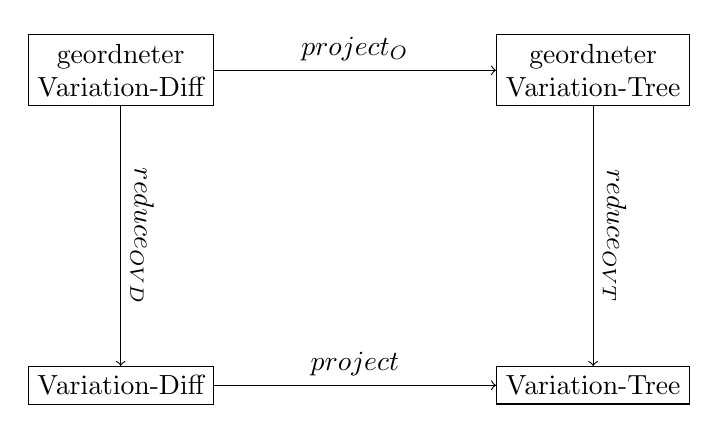
\begin{tikzpicture}
	\node[draw,align=center] (A) at (0,0) {geordneter\\
	Variation-Diff};
	\node[draw,align=center] (B) at (6,0) {geordneter\\
		Variation-Tree};
	\node[draw,align=center] (C) at (0,-4) {Variation-Diff};
	\node[draw,align=center] (D) at (6,-4) {Variation-Tree};
	\draw[->] (A) -- (B)  node[midway,sloped,above] {$project_O$} ;
	\draw[->] (C) -- (D)  node[midway,sloped,above] {$project$} ;
	\draw[->] (A) -- (C)  node[midway,sloped,above] {$reduce_{OVD}$} ;
	\draw[->] (B) -- (D)  node[midway,sloped,above] {$reduce_{OVT}$} ;
	\end{tikzpicture}
	\caption{Transformationen von geordneten Variation-Diff , geordneten Variation-Tree, Variation-Diff und Variation-Tree}
\end{figure}


\section{Parser}

Jetzt beschäftigen wir uns mit den Parsen, also wie Variation-Trees bzw. Variation-Diffs  aus mit C-Präprozessor-Direktiven annotiertem Code bzw. einem textbasierten Diff von solchem Code erstellt werden. Das Verständnis des Parsens ist, für das Verständnis des Unparsens von Bedeutung, da das Unparsen das Parsen invertiert. Dazu schauen wir uns den Parser-Algorithmus von Viegener~\cite{Viegener21} an, welcher das Parsen von Variation-Diffs aus textbasierten Diffs eingeführt hat.\\


Der unten stehender Algorithmus überführt einen textbasierten Diff in einen Variation-Diff. Dabei werden in dem Algorithmus einige Funktionen verwendet, die nicht so in der Definition vorkamen. Einer dieser Funktionen ist der Code-Typ dieser stellt dar, welche Rolle die Zeile in dem Diff hat. Es kann die Werte if, elif, else, code, oder endif haben. Bei dem Wert if ist gegeben, dass die Zeile eine der Präprozessor Anweisungen \#if, \#ifdef, oder \#ifndef hat. Bei dem Wert else ist in der Zeile die Präprozessor Anweisungen \#else, bei Wert elif ist  die Präprozessor Anweisungen \#elif und bei Wert endif ist  die Präprozessor Anweisungen \#endif gegeben. Wenn der Wert von Code-Typ code ist, dann enthält die Zeile keine Präprozessor Anweisungen, sondern normalen Code. Da Wert elif als Erweiterung betrachtet werden kann, wird auf sie nicht weiter in unserer Arbeit eingegangen. Der Code-Typ einer Zeile wird bei der Erstellung eines neuen Knotens in Knotentyp $\tau$ überführt. Der Code-Typ if wird in $\tau$ gleich \textsc{mapping}, der Code-Typ code wird in $\tau$ gleich \textsc{artifact} und der Code-Typ else wird in $\tau$ gleich \textsc{else} überführt. Der Code-Typ endif hat keine Überführung in Knotentyp $\tau$, diese Code-Type wird nur intern von dem Algorithmus verwendet. Eine andere Funktion ist der Diff-Typ, welcher für eine Zeile angibt, ob diese Zeile hinzugefügt wurde, entfernt wurde oder unverändert geblieben ist. Der Diff-Typ \textcolor{green}{+} sagt, dass die Zeile hinzugefügt wurde, \textcolor{orange}{--} sagt, dass die Zeile entfernt wurde und \textcolor{gray}{$\circ$} sagt, dass die Zeile unverändert geblieben ist. Der Diff-Typ wird, auch wie der Code-Typ, bei der Erstellung eines neuen Knotens in $\Delta$ überführt. Dabei wird \textcolor{green}{+} in \textcolor{green}{+}, \textcolor{orange}{--} in\textcolor{orange}{--} und \textcolor{gray}{$\circ$} in \textcolor{gray}{$\circ$} überführt. Der Variation-Diff hat noch einen Knoten welcher keine Widerspiegelung in dem textbasierten Diff enthält, das ist der Wurzelknoten. Der Wurzelknoten repräsentiert den ganzen textbasierten Diff. Er hat als einziger Knoten in dem Variation-Diff kein Elternknoten.


\begin{algorithm}[H]
	\SetAlgoLined
	\DontPrintSemicolon
	\KwData{ein textbasierter Diff}
	\KwResult{ein Variation-Diff}
	erstelle den Wurzelknoten\;
	initialisiere ein Stack/Keller $before$ mit dem Wurzelknoten\;
	initialisiere ein Stack/Keller $after$ mit dem Wurzelknoten\;
	\;
	\ForEach{Zeile in dem Patch/Diff}{
		$\delta$ $\leftarrow$ identifiziere Diff-Typ der Zeile\;
		$\gamma$ $\leftarrow$ identifiziere Code-Typ der Zeile\;
		$\sigma$ $\leftarrow$ identifiziere relevante Stacks mithilfe von  $\delta$\;
		\;
		\eIf{$\gamma$ = endif}{
		Entferne, solange Knoten von allen Stacks in $\sigma$, bis $\gamma$ = if entfernt wurde\;
		}{
			erstelle einen neuen Knoten mit $\delta$, $\gamma$ und gerichtete Kanten von Elternknoten aus $\sigma$ zu dem neu erstellten Knoten\;
			\If{$\gamma$ $\neq$ code}{
				füge den neuen Knoten $\sigma$ hinzu\;
			}
		}
	}
	\caption{Erstellung eines Variation-Diffs aus einem Patch}
\end{algorithm}
Der Algorithmus arbeitet wie folgt. Ganz am Anfang  wird der Wurzelknoten in Zeile 1 erstellt. Danach werden zwei Stacks erstellt und jeweils mit dem Wurzelknoten initialisiert, was in Zeilen 2 und 3 des Algorithmus 1 zu sehen ist. Die Stacks speichern dabei die Elternknoten. Ein Stack speichern die Elternknoten in davor Zustand und der anderer im danach Zustand. Beide Stacks werden mit Wurzelknoten befühlt, welcher den ganzen Diff repräsentiert und hat deshalb als einziger Knoten in Variation-Diff keinen Elternknoten. In Zeile 5 ist eine Schleife zu sehen, welche über alle Zeilen des textbasierten Diffs geht. Dabei wird für jede Zeile zuerst der Diff-Typ $\delta$ in Zeile 6 und dann der Code-Typ $\gamma$ in Zeile 7 ermittelt. In Zeile 8 werden die relevanten Stacks $\sigma$ anhand von Diff-Typ $\delta$ bestimmt, und zwar wie folgt:
\[ \sigma =
\begin{cases}
	\text{Stack } after      &, \quad \delta = \text{add}\\
	\text{Stack } before  &, \quad \delta = \text{remove}\\
	\text{Stacks } befor \text{ und } after &, \quad \delta = \text{none}
\end{cases}
\]
Diese Informationen werden zum einen dazu gebraucht für Algorithmus interne Berechnungen und zum anderen zur Erstellung von Knoten gebraucht. Danach in Zeile 10 kommen wir zu einer if-Abfrage. Wenn der Code-Typ der bearbeiteten Zeile endif entspricht, dann wird aus den relevanten Stacks in $\sigma$ solange Knoten entfernt bis man ein Knoten mit dem Code-Type $\gamma$ if entfernt hat. Falls beide Stacks relevant sind, muss der if-Knoten in beiden Stacks gefunden werden. Dieses Vorgehen ist Notwendig, da wenn eine endif-Anweisung kommt, muss der dazugehörige if-Block oder if-else-Block zu Ende sein. Das führt mit sich das die dazugehörigen if-Knoten und else-Knoten keine Elternknoten mehr sein können und aus den Stacks entfernt werden müssen. Wenn der Code-Typ nicht endif entspricht, kommen wir in den else-Teil ab Zeile 12 des Algorithmus 1. Dort wird zuerst ein neuer Knoten erstellt, dazu unter anderem wird Diff-Typ $\delta$ und Code-Typ $\gamma$ verwendet. Es werden auch Kanten von Elternknoten aus den Stacks von $\sigma$ zu diesen neuen Knoten erstellt. Als Nächstes wird in Zeile 14 überprüft, ob der erstellter Knoten nicht von Code-Typ code ist. Diese Abfrage ist nötig da nur solche Knoten ein Elternknoten sein können. Den Code-Typ endif kann dieser Knoten nicht haben, wegen der if-Abfrage in Zeile 10, welche nicht zulässt, dass ein Knoten mit diesem Typ zu dieser Stelle gelangen kann.  Wenn der Knoten nicht von Code-Typ code ist, dann wird dieser Knoten den relevanten Stacks aus $\sigma$ hinzugefügt, sonst wenn der Knoten, den Code-Type code hat, wird nichts gemacht.\\


Der vorgestellter Algorithmus ist für das Parsen von textbasierten Diffs, welche aus mit C-Präprozessor-Annotierten Code entstanden sind, zu Variation-Diffs ausgelegt aber es ist auch möglich den Algorithmus zum Parsen von C-Präprozessor-Annotiertem Code zu einem Variation-Tree zu verwenden. Wir reduzieren das Problem ein Variation-Tree zu parsen auf das Problem ein Variation-Diff zu parsen. Um das anstellen zu können, müssen wir zwei Sachen beachten. Zuerst wäre da die Anpassung der Eingabe, da wir C-Präprozessor-Annotierten Code haben aber der Algorithmus einen textbasierten Diff erwartet. Die zweite Sache wäre die Anpassung der Ausgabe, die Ausgabe des Algorithmus ist ein Variation-Diff, wir brauchen aber einen Variation-Tree. Um die Eingabe gerecht für den Algorithmus zu machen, müssen wir unseren C-Präprozessor-Annotierten Code in ein textbasiertes Diff verwandeln. Dazu bilden wir ein Diff mit unserem C-Präprozessor-Annotierten Code als Davor-Zustand und Danach-Zustand. Danach bekommen ein textbasiertes Diff in dem jede Zeile als unverändert markiert ist. Dabei hat jede Zeile dieses Diffs den Diff-Typ none. Da jetzt ein Diff gegeben ist, können wir auf den Diff den Algorithmus anwenden. Die Ausgabe ist dann ein Variation-Diff, welcher in ein Variation-Tree umgewandelt werden muss. Um dies anzustellen, bilden wir eine Projektion des Variation-Diffs auf den Davor- bzw. Danach-Zustand und bekommen einen Variation-Tree. Es ist irrelevant welcher von den beiden Zuständen genommen wird, da der Davor-Zustand gleich dem Danach-Zustand sein soll. Mit den gezeigten Zwischenschritten lässt sich dieser Algorithmus auch für das Parsen von C-Präprozessor-Annotierten Code zu Variation-Trees verwenden.\\


Wir wollen die Arbeitsweise des Algorithmus veranschaulichen. Dazu wenden wir den Algorithmus, auf das untenstehende, beispielhafte Stück C-Code mit C-Prüprozessor-Annotationen an und veranschaulichen das Vorgehen in der Abbildung 3.3. Diese Abbildung zeigt Kasten, welche den Variation-Diff und relevanten Stacks für angegebene Zeile aus dem C-Code unten, nachdem  der Algorithmus diese Zeile verarbeitet hat, enthalten. Hier ist ein C-Code gegeben. Wir brauchen aber ein textbasiertes Diff. Es wird wie in dem Abschnitt davor vorgegangen und dieser C-Code bildet ein Diff mit sich selbst, somit ist die nötige Eingabe gegeben.
\begin{figure}[h]
	\begin{itemize}
		\item[1 ] f();
		\item[2 ] \textbf{\#if}(A)
		\item[3 ] \hspace*{0.5cm} \textbf{\#if}(B||C)
		\item[4 ] \hspace*{1cm}g();
		\item[5 ] \hspace*{0.5cm}\textbf{\#else}
		\item[6 ] \hspace*{1cm}z();
		\item[7 ] \hspace*{0.5cm}\textbf{\#endif}
		\item[8 ] \hspace*{0.5cm}x();
		\item[9 ] \textbf{\#endif}
	\end{itemize}
	\caption{Beispiel für mit C-Präprozessor-Annotierten Code}
\end{figure}
Am Anfang des Algorithmus werden die Stacks erstellt und mit dem Wurzelknoten  initialisiert. Wir betrachten jetzt die Schleife, die über alle Zeilen des obigen Diffs geht. Wir kommen zur Zeile 1 des C-Codes, dort befindet sich eine normale Codezeile, welche nicht annotiert ist. Es ergibt sich, dass diese Zeile den Code-Typ code und den Diff-Typ none hat. Alle anderen Zeilen haben auch den Diff-Typ none, aus dem Grund wie dieser Diff gebildet wurde und deshalb lassen wir die Erwähnung des Diff-Typs für jede Zeile sein. Dasselbe gilt auch für die relevanten Stacks in $\sigma$, da alle Zeilen den Diff-Typ none haben, gilt für alle Zeilen auch die gleichen relevanten Stacks und das sind beide. Da diese Zeile nicht Code-Typ endif hat, wird ein Knoten mit Code-Type, Diff-Typ, Elternknoten aus den Stacks und dem Inhalt der Zeile erstellt und dem Variation-Diff hinzugefügt, wie das aussieht, ist in Abbildung 3.3 in dem Kasten \glqq Nach Z.1\grqq{} zu sehen. Der erstellter Knoten hat als Elternknoten den Wurzelknoten, wie es in den Stacks zu sehen ist. In Abbildung 3.3 im Kasten \glqq Nach Z.2\grqq{} ist der Variation-Diff und die relevanten Stacks nach der Bearbeitung der Zeile 2 zu sehen. Es wurde ein neuer Knoten erstellt, welcher eine if-Anweisung enthält und in beide Stacks wurden dieser Knoten hinzugefügt. Die Schleife wurde fast gleich wie im vorherigen Fall durchgelaufen, außer an der letzten if-Abfrage. Diese Abfrage war bei der Zeile 1 false dieses Mal, da wir keinen Code-Typ code haben, wird diese Abfrage ausgeführt und der neu erstellter Knoten den Stacks hinzugefügt. Der nächste Kasten rechts zeigt den Variation-Diff nach Zeile 3. Der Algorithmus ist genauso wie in vorherigen Fall vorgegangen. Weiter voran wird dem Variation-Diff im nächsten Schritt ein Code-Knoten hinzugefügt, da für die Erstellung dieses Knotens der Code selbst irrelevant ist, wurde hier genauso vorgegangen wie bei der Erstellung eines Code-Knotens in Zeile 1. In der Zeile 5 ist \#else als Anweisung gegeben. Diese Zeile hat den Code-Typ else und somit auch kein endif. Es wird in den else-Zweig der ersten Abfrage gegangen. Dort wird ein neuer Knoten mit Inhalt dieser Zeile erstellt. Der Knoten wird den Stacks hinzugefügt, da der Knoten else  als Code-Typ hat und nicht code, was die innere Abfrage erfüllt (Abb. 3.3 \glqq Nach Z.5\grqq{}). In der nächsten Zeile ist wieder eine Codezeile vorhanden und aus der wird ein Code-Knoten erstellt. Wie es danach aussieht, ist in Abbildung 3.3 \glqq Nach Z.6\grqq{} zu sehen. Danach in der Zeile 7 treffen wir das erste Mal auf die Anweisung \#endif, welche den Code-Typ endif hat. Damit gelangen wir in den if-Teil der ersten Abfrage, welcher sich in der Zeile 11 des Algorithmus 1 befindet. Der Algorithmus entfernt nun von beiden Stacks jeweils so lange Knoten, bis ein if-Knoten entnommen wurde. Dabei werden aus den Stacks die Knoten mit else und if(B||C) entnommen und übrig bleiben der if(A) Knoten und der Wurzelknoten. Dieser Schritt verändert den Variation-Diff nicht. Im nächsten Schritt treffen wir wieder auf eine Codezeile und erstellen einen Knoten und fügen den dem Variation-Diff hinzu, welcher in Abbildung 3.3 \glqq Nach Z.8\grqq{} zu sehen ist. In der Zeile 9 ist wieder ein \#endif und wir müssen wieder Knoten aus den Stacks entnehmen. Dieses Mal wird der Knoten if(A) entnommen und es bleibt nur der Wurzelknoten übrig. Damit wäre die Arbeit des Algorithmus zu Ende und wir haben als Rückgabewert einen Variation-Diff erhalten. Wir brauchen einen Variation-Tree statt eines Variation-Diffs welchen wir bekommen habe. Dazu müssen wir noch eine Projektion auf den Zustand davor oder danach bilden. Schlussendlich erhalten wir einen Variation-Tree, welcher genauso aufgebaut ist, wie der Variation-Diff aus der Abbildung 3.3 Kasten \glqq Nach Z.8\grqq{}.
\begin{figure}[H]
	\centering
	\resizebox{0.9999\textwidth}{!}{
	\begin{tikzpicture}
		\node (A) at (-1,0) {\fbox {
				\begin{tikzpicture}
					\node[draw,diamond,fill=lightgray,thick] {root}
					child {node[draw,circle,thick] {f();}};
					\node at (-0.7,2.2) {davor};
					\node[rectangle split, rectangle split parts=2,draw, anchor=center] at (-0.7,1.5) {\nodepart{two} root };
					\node at (0.7,2.2) {danach};
					\node[rectangle split, rectangle split parts=2,draw, anchor=center] at (0.7,1.5) {\nodepart{two} root };
				\end{tikzpicture}
			}
		};
		\node (B) at (3,0) {\fbox {
				\begin{tikzpicture}
					\node[draw,diamond,fill=lightgray,thick] {root}
					child {node[draw,circle,thick] {f();}}
					child {node[draw,rectangle,thick] {\textbf{if}(A)}};
					\node at (-0.7,2.8) {davor};
					\node[rectangle split, rectangle split parts=3,draw, anchor=center] at (-0.7,1.8) {\nodepart{two} \textbf{if}(A) \nodepart{three} root};
					\node at (0.7,2.8) {danach};
					\node[rectangle split, rectangle split parts=3,draw, anchor=center] at (0.7,1.8) {\nodepart{two} \textbf{if}(A) \nodepart{three} root};
				\end{tikzpicture}
			}
		};
		\node (C) at (7,0) {\fbox {
				\begin{tikzpicture}
					\node[draw,diamond,fill=lightgray,thick] {root}
					child {node[draw,circle,thick] {f();}}
					child {node[draw,rectangle,thick] {\textbf{if}(A)}
						child {node[draw,rectangle,thick] {\textbf{if}(B$\lor$C)}}
					};
					\node at (-0.7,2.8) {davor};
					\node[rectangle split, rectangle split parts=3,draw, anchor=center] at (-0.7,1.8) {\nodepart{two} \textbf{if}(A) \nodepart{three} root};
					\node at (0.7,2.8) {danach};
					\node[rectangle split, rectangle split parts=3,draw, anchor=center] at (0.7,1.8) {\nodepart{two} \textbf{if}(A) \nodepart{three} root};
				\end{tikzpicture}
			}
		};
		\node (D) at (12,0) {\fbox {
				\begin{tikzpicture}
					\node[draw,diamond,fill=lightgray,thick] {root}
					child {node[draw,circle,thick] {f();}}
					child {node[draw,rectangle,thick] {\textbf{if}(A)}
						child {node[draw,rectangle,thick] {\textbf{if}(B$\lor$C)}
							child { node[draw,circle,thick] {g();}}
						}
					};
					\node at (2.5,0.7) {davor};
					\node[rectangle split, rectangle split parts=4,draw, anchor=center] at (2.5,-0.6) {\nodepart{two} \textbf{if}(B$\lor$C)  \nodepart{three} \textbf{if}(A) \nodepart{four} root};
					\node at (2.5,-2.3) {danach};
					\node[rectangle split, rectangle split parts=4,draw, anchor=center] at (2.5,-3.7) {\nodepart{two} \textbf{if}(B$\lor$C)  \nodepart{three} \textbf{if}(A) \nodepart{four} root};
				\end{tikzpicture}
			}
		};
		\node (E) at (-0.5,-7.5) {\fbox {
				\begin{tikzpicture}
					\node[draw,diamond,fill=lightgray,thick] {root}
					child {node[draw,circle,thick] {f();}}
					child {node[draw,rectangle,thick] {\textbf{if}(A)}
						child {node[draw,rectangle,thick] {\textbf{if}(B$\lor$C)}
							child { node[draw,circle,thick] {g();}}
							child { node[draw,rectangle,thick] {\textbf{else}}}
						}
					};
					\node at (3,0.95) {davor};
					\node[rectangle split, rectangle split parts=5,draw, anchor=center] at (3,-0.6) {\nodepart{two}\textbf{else}   \nodepart{three} \textbf{if}(B$\lor$C) \nodepart{four} \textbf{if}(A) \nodepart{five} root};
					\node at (3,-2.3) {danach};
					\node[rectangle split, rectangle split parts=5,draw, anchor=center] at (3,-3.9) {\nodepart{two}\textbf{else}   \nodepart{three} \textbf{if}(B$\lor$C) \nodepart{four} \textbf{if}(A) \nodepart{five} root};
				\end{tikzpicture}
			}
		};
		\node (F) at (6,-7.5) {\fbox {
				\begin{tikzpicture}
					\node[draw,diamond,fill=lightgray,thick] {root}
					child {node[draw,circle,thick] {f();}}
					child {node[draw,rectangle,thick] {\textbf{if}(A)}
						child {node[draw,rectangle,thick] {\textbf{if}(B$\lor$C)}
							child { node[draw,circle,thick] {g();}}
							child { node[draw,rectangle,thick] {\textbf{else}}
								child { node[draw,circle,thick] {z();}}
							}
						}
					};
					\node at (3,0.65) {davor};
					\node[rectangle split, rectangle split parts=5,draw, anchor=center] at (3,-0.9) {\nodepart{two}\textbf{else}   \nodepart{three} \textbf{if}(B$\lor$C) \nodepart{four} \textbf{if}(A) \nodepart{five} root};
					\node at (3,-2.85) {danach};
					\node[rectangle split, rectangle split parts=5,draw, anchor=center] at (3,-4.5) {\nodepart{two}\textbf{else}   \nodepart{three} \textbf{if}(B$\lor$C) \nodepart{four} \textbf{if}(A) \nodepart{five} root};
				\end{tikzpicture}	
			}
		};
		\node (G) at (12.5,-7.5) {\fbox {
				\begin{tikzpicture}
					\node[draw,diamond,fill=lightgray,thick] {root}
					child {node[draw,circle,thick] {f();}}
					child {node[draw,rectangle,thick] {\textbf{if}(A)}
						child {node[draw,rectangle,thick] {\textbf{if}(B$\lor$C)}
							child { node[draw,circle,thick] {g();}}
							child { node[draw,rectangle,thick] {\textbf{else}}
								child { node[draw,circle,thick] {z();}}
							}
						}
						child { node[draw,circle,thick] {x();}}
					};
					\node at (3,0.05) {davor};
					\node[rectangle split, rectangle split parts=3,draw, anchor=center] at (3,-0.9) {\nodepart{two} \textbf{if}(A) \nodepart{three} root};
					\node at (3,-3.5) {danach};
					\node[rectangle split, rectangle split parts=3,draw, anchor=center] at (3,-4.5) {\nodepart{two} \textbf{if}(A) \nodepart{three} root};
				\end{tikzpicture}
			}
		};
		\draw[->,thick] (A) --(B);
		\draw[->,thick] (B) --(C);
		\draw[->,thick] (C) --(D);
		\draw[thick] (D) |- (-0.5,-3.5);
		\draw[->,thick] (-0.5,-3.5) --(E);
		\draw[->,thick] (E) --(F);
		\draw[->,thick] (F) --(G);
		\node (a) at (-1,2.5) {Nach Z.1};
		\node (b) at (3,2.8) {Nach Z.2};
		\node (c) at (6.8,3.5) {Nach Z.3};
		\node (d) at (11.5,3.3) {Nach Z.4};
		\node (e) at (-0.5,-11.1) {Nach Z.5};
		\node (f) at (5.7,-11.6) {Nach Z.6};
		\node (g) at (12,-11.5) {Nach Z.8};
	\end{tikzpicture}
	}
	\caption{Beispiel für den Parsen Algorithmus von Viegener}
\end{figure}


Dieser Algorithmus kann sowohl gewöhnliche Variation-Diffs nach Definition 3.2 als auch geordneten Variation-Diffs nach Definition 3.5 erstellen. Das ist möglich, da die Reihenfolge der Kindknoten in Zeile 12 festgelegt wird.  \\

Jetzt wissen wir wie der Parser von Viegener funktioniert und der Parser auch für mehr als nur eine Definition von Variation-Diff zu gebrauchen ist. Dies können wir uns zunutze machen, wenn wir eine eigene Definition von Variation-Diff und Variation-Tree ausarbeiten werden. Es ist nun an der Zeit zu sehen, welche Informationen durch das Parsen und der Definitionen nach verloren gehen und wie wir diese Informationen zurückbekommen können.

\section{Verlorengehende Informationen und deren Wiederherstellung}

Nachdem wir uns mit dem Beschäftigt haben, was Variation-Trees und Variation-Diffs sind und wie dieser aus mit C-Präprozessor-Annotierten Code und textbasierten Diffs erzeugt werden. Werden wir uns damit auseinandersetzen welche Informationen während des Parsens verloren gehen. Also welche Informationen sind im mit C-Präprozessor-Annotierten Code bzw. textbasierten Diff erhalten, aber nach dem Parsen nicht in Variation-Tree bzw. Variation-Diff zu finden sind. Und wie wir diese Informationen zurückbekommen können, um das Unparsen zu bewerkstelligen. Die verlorengehende Informationen sind die Ordnung der Zeilen, die Position von  Zeilen mit einem \#endif innerhalb von textbasierten Diff bzw. mit C-Präprozessor-Annotierten Code und der Inhalt aller Zeilen inklusive der Zeilen mit \#endif und \#else.\\

Der Definition von Variation-Tree bzw. Variation-Diff nach haben, die Kinder eines Knotens keine Reihenfolge. Deshalb können wir nicht wissen, bei dem Unparsen welcher Knoten zuerst kommt und welcher danach. Zum Beispiel ein Variation-Tree kann mehrdeutig verstanden wäre, was für uns nicht zu gebrauchen ist.
\begin{figure}[H]
	\begin{tikzpicture}
		\node[draw,diamond,fill=lightgray,thick] {root}
		child {node[draw,circle,thick] {foo()}}
		child {node[draw,circle,thick] {bar()} };	
		\node[draw,align=left] (a) at (-1,-3) {foo()\\bar()};
		\node at (0,-3) {oder};
		\node[draw,align=left] (a) at (1,-3) {bar()\\foo()};
	\end{tikzpicture}
\end{figure}
Um das Problem umzugehen, wie wir schon erwähnt haben, verwenden wir statt der normalen Definition von Variation-Tree und Variation-Diff die Definition von geordneten Variation-Tree und geordneten Variation-Diff. Diese Definition hat eine Ordnung bei den Kinderknoten. Deshalb kann sie uns eine eindeutige Reihenfolge geben, so das keine Mehrdeutigkeiten in Bezug auf das wie die Knoten eingeordnet sind vorkommt. Das Umsetzen dieser Definition von dem Parser stellt für uns keine Schwierigkeiten dar. Die Definitionen von normalen Variation-Tree bzw. Variation-Diff unterscheiden sich von geordneten Variation-Tree bzw. geordneten Variation-Diff nur um die Ordnung O. Was zu Folge hat das alles andere so wie gewohnt umgesetzt werden kann. Die Ordnung selbst muss dann gesetzt werde, wenn ein neuer Knoten entsteht und er seine Eltern bekommt. Dies findet in der Zeile 12 des Algorithmus 1. Dort stehen keine genaueren Angaben zu Erstellung des Knotens, also kann diese Zeile auch um die Setzung der Ordnung erweitert werden. Damit haben wir unseren ersten Informationsverlust beseitigt.\\

Als nächstes Beschäftigen wir ums mit dem  Verlust der Position von \#endif. Es gibt keinen Knoten innerhalb von Variation-Trees und Variation-Diffs , welcher \#endif repräsentiert. Deshalb wissen wir nicht, wo sich die Zeilen mit \#endif befinden müssen wenn wir das gegebene unparsen. Zu Beschaffung diese Information muss die Position von \#endif aus der gegebener Information rekonstruiert werden. In dieser Beschreibung wird einfachheitshalber so gehandelt, als gäbe es ein Knoten für \#endif.  Um zu bestimmen, ob ein Knoten als sein letztes Kinderknoten ein \#endif besitzen wird, müssen wir prüfen ob der Knoten $\tau$ gleich mapping hat. Wenn das zutrifft, wird ein Dummyknoten als neuer letzter Kindknoten zu diesem Knoten hinzugefügt. Nach dieser Handlung wissen wir, dass die Zeile mit dem \#endif nach dem Inhalt allen anderen Kinderknoten und dessen Unterbäumen kommt. Damit haben wir auch eine Möglichkeit diesen Information-Verlust zu beseitigen.\\

Als letztes müssen wir uns damit beschäftigen wie wir den Inhalt aller Zeilen aus Variation-Tree oder Variation-Diff bekommen können. Bei Zeilen mit \#endif und \#else wäre es möglich mit Heuristiken zu arbeiten, da die Einrückung von \#endif und \#else im Falle von C-Präprozessor nicht dazu führt, das Code fehlerhaft wird. Es wäre möglich eine Heuristik, wie z.B. das \#endif  und \#else so weit eingerückt sind, wie der dazugehörige if oder das \#else und \#endif immer am Zeilenanfang sind, zu verwenden. Bei der Verwendung einer Heuristik, können wir nicht die exakte Gleichheit garantieren, erfordert aber keine extra Aufwände. Dazu könnten Kommentare in diesen Zeilen nicht wiederbekommen werden. Bei Knoten mit $\tau$ gleich artifact, könnte man so vorgehen, das man in Label die Zeile abspeichert. Der Definition von Label nach werden dort entweder ein Implementierungsartefakt oder eine aussagenlogische Formel gespeichert. Ein Implementierungsartefakt kann dabei mehr als nur die Codezeile sein. Ein Implementierungsartefakt ist dabei  eine identifizierbare Einheit mit beliebiger Granularität innerhalb eines Softwareprojekts~\cite{BTS+:ESECFSE22}. Unsere Arbeit ist darauf ausgelegt, dass wir einen Unparser bereitstellen, welcher aus Variation-Trees bzw. Variation-Diffs mit C-Präprozessor-Annotierten Code bzw. textbasiertes Diff erstellt. Wir konnten fordern, dass das Label als Implementierungsartefakt die Codezeile abspeichert. Für Knoten mit $\tau$ gleich else oder mapping würde das aber nicht funktionieren. Für Knoten mit $\tau$ gleich else wird der Definition nach überhaupt kein Label gespeichert. Für Knoten mit $\tau$ gleich mapping wird das Label eine aussagenlogische Formel speichern, aber die Bedingungen in der C-Präprozessor-Annotation sind nicht immer eine aussagenlogische Formel und muss deshalb durch boolean abstraction~\cite{BTS+:ESECFSE22} in solche umgewandelt werden. Das kann z.B. so aussehen: \#if A(x) > 3 ist gegeben und nach boolean abstraction sieht es dann so aus \#if A\_\_LB\_\_x\_\_RB\_\_GT\_\_3. Dabei ist eine zurück Umwandlung nicht garantiert, da wir nicht sicher sein können das z.B  A\_\_LB\_\_x\_\_RB\_\_GT\_\_3 nicht als ein Variablenname gewählt wurde und damit keine Umwandlung benötigt. Es ergibt sich, dass das Label nur für $\tau$ gleich artifact gut die Zeile speichern kann, bei den anderen Zeilen gibt es Schwierigkeiten. Um diese Informationen auch im Variation-Tree und Variation-Diff zu haben, müssen wir diese Informationen explizit speichern. Die Definitionen von Variation-Tree, Variation-Diff, geordneten Variation-Tree und geordneten Variation-Diff sehen aber dafür nichts vor. Deshalb müssen wir die Definition von Variation-Diff bzw. geordneten Variation-Tree und Variation-Diff bzw. geordneten Variation-Diff erweitern. Obwohl wir für $\tau$ gleich artifact die Zeile in dem Label speichern können, werden wir wegen der Einheitlichkeit alle Zeile in der Erweiterung speichern und die nicht unterscheiden.
Wir erweitern die Definitionen wie folgt:
\begin{definition}
	Ein \textsc{speichernder Variation-Tree} $(V,E,r,\tau,l,M) $ ist für V, E, r, $\tau$ und l so definiert wie in der Definition 3.1 und M : V $\rightarrow$ (String ,String) speichert in der ersten Stelle des Tupels die Zeile, welche der Knoten darstellt und an der zweiten Stelle wird für Knoten mit $\tau$ gleich mapping die dazugehörige Zeile mit \#endif gespeichert, für die restlichen Knoten wird dort Null gespeichert.
\end{definition}
\begin{definition}
	Ein \textsc{speichernder Variation-Diff} $(V,E,r,\tau,l,\Delta,M) $ ist für V, E, r, $\tau$, l und $\Delta$ so definiert wie in der Definition 3.2 und M : V $\rightarrow$ (String ,String) speichert in der ersten Stelle des Tupels die Zeile, welche der Knoten darstellt und an der zweiten Stelle wird für Knoten mit $\tau$ gleich mapping die dazugehörige Zeile mit \#endif gespeichert, für die restlichen Knoten wird dort Null gespeichert.
\end{definition}
\begin{definition}
	Ein \textsc{geordneter, speichernder Variation-Tree} $(V,E,r,\tau,l,O,M) $ ist für V, E, r, $\tau$, l und O so definiert wie in der Definition 3.5 und M : V $\rightarrow$ (String ,String) speichert in der ersten Stelle des Tupels die Zeile, welche der Knoten darstellt und an der zweiten Stelle wird für Knoten mit $\tau$ gleich mapping die dazugehörige Zeile mit \#endif gespeichert, für die restlichen Knoten wird dort Null gespeichert.
\end{definition}
\begin{definition}
	Ein \textsc{geordneter, speichernder Variation-Diff} $(V,E,r,\tau,l,O_{before},O_{after},M) $ ist für V, E, r, $\tau$, l, $O_{before}$ und $O_{after}$ so definiert wie in der Definition 3.6 und M : V $\rightarrow$ (String ,String) speichert in der ersten Stelle des Tupels die Zeile, welche der Knoten darstellt und an der zweiten Stelle wird für Knoten mit $\tau$ gleich mapping die dazugehörige Zeile mit \#endif gespeichert, für die restlichen Knoten wird dort Null gespeichert.
\end{definition}
Dazu nachdem wir die neuen Variation-Trees und Variation-Diffs definiert haben, müssen wir noch entsprechende Projektionen definieren.
\begin{definition}
	Die Projektion $project_{M}$($D,t$) für das speichernde Variation-Diff ist das Entfernen von $\Delta$, M und der Knoten und Kanten, welche zu der Zeit t nicht vorhanden sind. $project_{M}$$((V,E,r,\tau,l,\Delta,M),t) := (\{v \in V | $\textsc{exists}$(t,\Delta(v))\},\{e \in E | $\textsc{exists}$(t,\Delta(e))\},r,\tau,l,M)$
\end{definition}
\begin{definition}
	Die Projektion $project_{OM}$($D,t$) für das geordnete, speichernde Variation-Diff ist das Entfernen von $\Delta$, M und der Knoten und Kanten, welche zu der Zeit t nicht vorhanden sind. Dazu wird nur der Zeit entsprechende Ordnung $O_t$ behalten.\\ $project_{OM}$$((V,E,r,\tau,l,\Delta,O_{before},O_{after},M),t)\\ := (\{v \in V | $\textsc{exists}$(t,\Delta(v))\},\{e \in E | $\textsc{exists}$(t,\Delta(e))\},r,\tau,l,O_t,M)$
\end{definition}
Da wir die Definitionen erweitert haben, ist es  möglich die speichernden Variation-Trees bzw. Variation-Diffs in normale Variation-Trees bzw. Variation-Diffs und geordnete, speichernden Variation-Trees bzw. Variation-Diffs in geordnete Variation-Trees bzw. Variation-Diffs umzuwandeln. 
\begin{definition}
	$reduce_{MVT}$ wandelt ein speicherndes Variation-Tree (Definition 3.11) in ein normales Variation-Tree (Definition 3.1) \\
	$reduce_{MVT}((V,E,r,\tau,l,M)) := (V,E,r,\tau,l)$.
\end{definition}
\begin{definition}
	$reduce_{MVD}$ wandelt ein speicherndes Variation-Diff (Definition 3.12) in ein normales Variation-Diff (Definition 3.2) \\
	$reduce_{MVD}((V,E,r,\tau,l,\Delta,M)) := (V,E,r,\tau,l,\Delta)$
\end{definition}
\begin{definition}
	$reduce_{MOVT}$ wandelt ein geordnetes, speicherndes Variation-Tree (Definition 3.13) in ein geordnetes Variation-Tree (Definition 3.5) \\
	$reduce_{MOVT}((V,E,r,\tau,l,O,M)) := (V,E,r,\tau,l,O)$
\end{definition}
\begin{definition}
	$reduce_{MOVD}$ wandelt ein geordnetes, speicherndes Variation-Diff (Definition 3.14) in ein geordnetes Variation-Diff (Definition 3.6) \\
	$reduce_{MOVD}((V,E,r,\tau,l,\Delta,O_{before},O_{after},M)) := (V,E,r,\tau,l,\Delta,O_{before},O_{after})$
\end{definition}
Es bleibt uns nur noch zu zeigen das die Reihenfolge der Anwendung von $project$ und $reduce$ irrelevant ist. Dann zusammen mit den gezeigten aus Kapitel 3.1 ist die Abbildung 3.4 gegeben, welche eine Erweiterung der Abbildung 3.1 ist. Die Abbildung 3.4 veranschaulicht die Transformationen von geordneten speichernden Variation-Trees, geordneten speichernden Variation-Diffs,  speichernden Variation-Trees, speichernden Variation-Diffs, geordneten Variation-Trees, geordneten Variation-Diffs, normalen Variation-Trees und normalen Variation-Diffs.
\begin{lemma}
	Für einen speichernden Variation-Diff D und eine Zeit $t \in \{before, after\}$ gilt $reduce_{MVT}(project_M(D,t)) = project(reduce_{MVD}(D),t)$.
\end{lemma}
\begin{proof}
	$
	reduce_{MVT}(project_M(D,t))\\ 
	= reduce_{MVT}(project_M((V,E,r,\tau,l,\Delta,M),t))\\
	= reduce_{MVT}((\{v \in V | \textsc{exists}(t,\Delta(v))\},\{e \in E | \textsc{exists}(t,\Delta(e))\},r,\tau,l,M))\\
	= (\{v \in V | \textsc{exists}(t,\Delta(v))\},\{e \in E | \textsc{exists}(t,\Delta(e))\},r,\tau,l)\\ 
	= project((V,E,r,\tau,l,\Delta),t)\\ 
	= project(reduce_{MVD}(V,E,r,\tau,l,\Delta,M),t)\\ 
	= project(reduce_{MVD}(D),t)\\
	$
\end{proof}
\begin{lemma}
	Für einen geordneten, speichernden Variation-Diff D und eine Zeit $t \in \{before, after\}$ gilt $reduce_{MOVT}(project_{OM}(D,t)) = project_{O}(reduce_{MOVD}(D),t)$.
\end{lemma}
\begin{proof}
	$
	reduce_{MOVT}(project_{OM}(D,t))\\ 
	= reduce_{MOVT}(project_{OM}((V,E,r,\tau,l,\Delta,O_{before},O_{after},M),t))\\
	= reduce_{MOVT}((\{v \in V | \textsc{exists}(t,\Delta(v))\},\{e \in E | \textsc{exists}(t,\Delta(e))\},r,\tau,l,O_t))\\
	= (\{v \in V | \textsc{exists}(t,\Delta(v))\},\{e \in E | \textsc{exists}(t,\Delta(e))\},r,\tau,l,O_t)\\ 
	= project_O((V,E,r,\tau,l,\Delta,O_{before},O_{after}),t)\\ 
	= project_O(reduce_{MOVD}(V,E,r,\tau,l,\Delta,O_{before},O_{after},M),t)\\ 
	= project_O(reduce_{MOVD}(D),t)\\
	$
\end{proof}
Nach dem Ganzen ergibt sich, ein folgendes Schaubild:
\begin{figure}[H]
	\centering
	\resizebox{0.95\textwidth}{!}{
	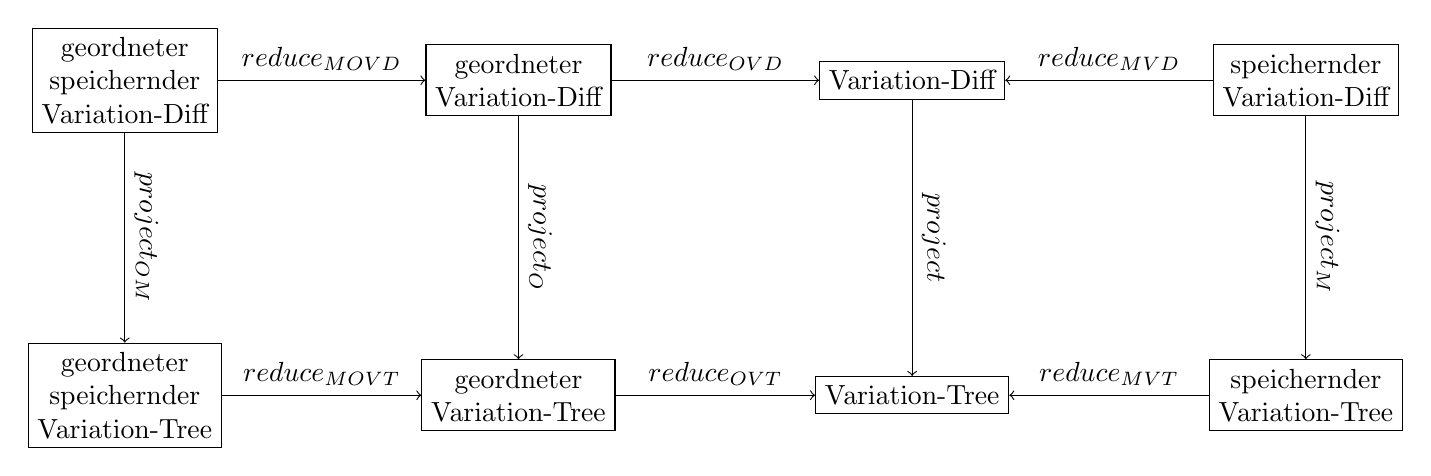
\begin{tikzpicture}
		\node[draw,align=center] (E) at (0,0) {geordneter\\speichernder\\
			Variation-Diff};
		\node[draw,align=center] (F) at (0,-4) {geordneter\\speichernder\\
			Variation-Tree};
		\node[draw,align=center] (A) at (5,0) {geordneter\\
			Variation-Diff};
		\node[draw,align=center] (B) at (5,-4) {geordneter\\
			Variation-Tree};
		\node[draw,align=center] (C) at (10,0) {Variation-Diff};
		\node[draw,align=center] (D) at (10,-4) {Variation-Tree};
		\node[draw,align=center] (G) at (15,0) {speichernder\\
			Variation-Diff};
		\node[draw,align=center] (H) at (15,-4) {speichernder\\
			Variation-Tree};
		\draw[->] (A) -- (B)  node[midway,sloped,above] {$project_O$} ;
		\draw[->] (C) -- (D)  node[midway,sloped,above] {$project$} ;
		\draw[->] (A) -- (C)  node[midway,sloped,above] {$reduce_{OVD}$} ;
		\draw[->] (B) -- (D)  node[midway,sloped,above] {$reduce_{OVT}$} ;
		\draw[->] (E) -- (F)  node[midway,sloped,above] {$project_{OM}$} ;
		\draw[->] (E) -- (A)  node[midway,sloped,above] {$reduce_{MOVD}$} ;
		\draw[->] (F) -- (B)  node[midway,sloped,above] {$reduce_{MOVT}$} ;
		\draw[->] (G) -- (H)  node[midway,sloped,above] {$project_{M}$} ;
		\draw[->] (G) -- (C)  node[midway,sloped,above] {$reduce_{MVD}$} ;
		\draw[->] (H) -- (D)  node[midway,sloped,above] {$reduce_{MVT}$} ;
	\end{tikzpicture}
	}
	\caption{Transformationen von verschiedenen Variation-Trees und Variation-Diffs}
\end{figure}
Nachdem wir uns mit den neuen Definitionen beschäftigt haben, müssen wir noch den Parsen anpassen. Damit der Parser auch diese Definitionen umsetzen kann. Dazu muss man die Zeile 11 des Algorithmus etwas erweitern, damit der Algorithmus den Knoten mit $\gamma$ = if sich merkt. Dazu muss man noch eine neue Zeile zu dem Algorithmus zufügen und das ist die Zeile 12 des Algorithmus 2. Dort wird ein Tupel mit dazugehöriger Zeile des Knotens und 
der Zeile, mit dem \#endif, erstellt. Dann wird diese Tupel in M für den gemerkten Knoten gespeichert. Alle anderen Zeilen werden für ihre Knoten jeweils in Zeile 15 des Algorithmus 2 gespeichert. Dort wird ein Tupel mit der Zeile und Null erstellt und für den neu erstellten Knoten gespeichert. Damit sind wir in der Lage die neuen Definitionen auch aus mit C-Präprozessor-Annotierten Code und textbasierten Diffs zu erzeugen. 

\begin{algorithm}[H]
	\SetAlgoLined
	\DontPrintSemicolon
	\KwData{ein textbasierter Diff}
	\KwResult{ein Variation-Diff}
	erstelle den Wurzelknoten\;
	initialisiere ein Stack/Keller $before$ mit dem Wurzelknoten\;
	initialisiere ein Stack/Keller $after$ mit dem Wurzelknoten\;
	\;
	\ForEach{Zeile in dem Patch/Diff}{
		$\delta$ $\leftarrow$ identifiziere Diff-Typ der Zeile\;
		$\gamma$ $\leftarrow$ identifiziere Code-Typ der Zeile\;
		$\sigma$ $\leftarrow$ identifiziere relevante Stacks mithilfe von  $\delta$\;
		\;
		\eIf{$\gamma$ = endif}{
			Entferne, solange Knoten von allen Stacks in $\sigma$, bis ein Knoten v $\gamma$ = if entfernt wurde\;
			M(v) $\leftarrow$ (M(v)[0],Zeile)\;
		}{
			erstelle einen neuen Knoten v mit $\delta$, $\gamma$ und gerichtete Kanten von Elternknoten aus $\sigma$ zu dem neu erstellten Knoten\;
			M(v) $\leftarrow$ (Zeile,Null)\;
			\If{$\gamma$ $\neq$ code}{
				füge den neuen Knoten $\sigma$ hinzu\;
			}
		}
	}
	\caption{Erstellung eines Variation-Diffs, welcher sich \#else und \#endif merkt, aus einem Patch}
\end{algorithm}
Mit der Erweiterung der Definitionen können wir den Inhalt der Zeile mit \#endif oder \#else bekommen und damit ist dieser Informationsverlust auch beseitigt.\\

%Als Letztes müssen wir uns damit befassen, wie wir den Inhalt der Zeilen bekommen. Der Definition von Label nach werden dort entweder ein Implementierungsartefakt oder eine aussagenlogische Formel gespeichert. Ein Implementierungsartefakt kann dabei mehr als nur die Codezeile sein. Ein Implementierungsartefakt ist dabei  eine identifizierbare Einheit mit beliebiger Granularität innerhalb eines Softwareprojekts~\cite{BTS+:ESECFSE22}. Dazu sind Bedingungen in if-Anweisungen sind nicht immer als aussagenlogische Formeln gegeben und werden deshalb mithilfe von boolean abstraction in solche umgewandelt~\cite{BTS+:ESECFSE22}. Das kann z.B. so aussehen: \#if A(x) > 3 ist gegeben und nach boolean abstraction sieht es dann so aus \#if A\_\_LB\_\_x\_\_RB\_\_GT\_\_3. Dabei ist eine zurück Umwandlung nicht garantiert, da wir nicht sicher sein können das z.B  A\_\_LB\_\_x\_\_RB\_\_GT\_\_3 nicht als ein Variablenname gewählt wurde und damit keine Umwandlung benötigt. Unsere Arbeit ist darauf ausgelegt, dass wir einen Unparser bereitstellen, welcher aus Variation-Trees bzw. Variation-Diffs mit C-Präprozessor-Annotierten Code bzw. textbasiertes Diff erstellt. Aus dem Grund, da wir so spezialisiert sind, fordern wir das Label als Implementierungsartefakt die Codezeile abspeichert und die aussagenlogischen Formeln trotzt dem boolean abstraction sich zu if-Bedingungen invertieren lassen. Mit diesen Forderungen beseitigen wir auch den letzten Informationsverlust.\\

Nachdem wir herausgefunden haben, welche für das Unparsen relevante Information verloren geht und wie man diese Information Zurück bekommen kann, sind wir in der Lage das alles zu nutzen, um einen Algorithmus zum Unparsen zu entwickeln.


\section{Unparsing}

%Im Baum stellen Knoten Blöcke dar, Tiefensuche geht alle blöcke eiser zweigt zuerst durch dann zum nächsten so entsteht wieder der Text


Nachdem wir festgestellt haben welche Informationen während des Parsens verloren gehen und wie diese zurückzubekommen sind, sind wir in der Lage das Unparsen zu bewerkstelligen. Darüber geht es in diesem Unterkapitel. Wir stellen unseren Algorithmus für das Unparsen von speichernden, geordneten Variation-Trees und ein Vorgehen zum Unparsen von speichernden, geordneten Variation-Diffs.\\

%Damit unser Algorithmus korrekt funktioniert müssen paar Sachen beachtet werden. Als erstes gehen wir davon aus das die Reihenfolge der Knoten auch die Reihenfolge der Zeilen in dem Ergebnis des Unparsers widerspiegelt. Wenn ein Kindknoten A vor dem Kindknoten B aufgelistet wird bedeutet, dass das der Inhalt alle Knoten die einen Teilbaum mit Kindknoten A als Wurzel bilden vor dem Inhalt des Kindknoten B kommt. Als zweites muss man beachtet das Variation-Trees und Variation-Diffs keine Speicherung der Information über \#endif vorsehen. Unser Algorithmus kann zwar bestimmen an welchen Stellen ein \#endif kommen soll, aber er kann nicht die genauere Entfernung von Zeilenanfang wissen. Aus diesem Grund muss man hier entweder mit einer Heuristik arbeiten oder die Implementierung von Variation-Tree und Variation-Diff so modifizieren das diese Informationen gespeichert werden und wenn benötigt abgerufen.

Unser Algorithmus ist der Algorithmus 3 und ist nur für das Unparsen von speichernden, geordneten Variation-Tree zu einem mit C-Präprozessor-Annotierten Code bestimmt. Wenn man M aus dem Algorithmus durch eine Heuristik ersetzt, ist es auch möglich mithilfe unseres Algorithmus geordnete Variation-Trees umzuparsen. Der Algorithmus basiert auf der Tiefensuche. Ein Variation-Tree ist ein Baum, dessen Knoten die Zeilen des  mit C-Präprozessor-Annotierten Codes enthalten. Dabei wenn ein Knoten Kinderknoten hat, bedeutet es das dieser Knoten $\tau$ gleich mapping oder $\tau$ gleich else hat. Dazu wissen wir dadurch, dass die Anweisungen im Kinderknoten von der Anweisung des Elternknotens eingeschlossen werden. Wegen so einer Anordnung ist die Verwendung von Tiefensuche von Vorteil. Die Tiefensuche besucht alle Knoten effizient und dazu geht die Tiefensuche zunächst ein Pfad vollständig in die Tiefe, bevor abzweigende Pfade beschritten werden. Die Auswahl des nächsten Knotens welcher besucht wird muss etwas geändert werden, damit die Pfade der Reihenfolge nach beschritten werden. Dazu werden die Kinderknoten eines Knotens den Stack in umgedrehter Reihenfolge hinzugefügt. Es ergibt sich, dass der letzte Kinderknoten auch als letzter drankommt und der erster als erster. Das zusammen ergibt, das unser Algorithmus die Knoten so besucht wie die in den Knoten enthaltene Zeilen angeordnet werden müssen.\\

Jetzt schauen wir und den Algorithmus an, nachdem wir sein Konzept besprochen haben. In Zeile 1 des Algorithmus 3 wird ein Stack initialisiert, so wie in der Tiefensuche. Danach in Zeile 2 wird ein String initialisiert, in dem am Ende der gesamte annotierter Code gespeichert wird. Von Zeile 3 bis Zeile 10 werden die Kinderknoten des Wurzelknotens auf den Stack gelegt. Das muss extra gemacht werden, da der Wurzelknoten keine Zeile enthält als Label, sondern true. Damit würde er das Ergebnis verfälschen. Genauer betrachtet wird folgendes gemacht, in der Zeile 3 werden die Kinderknoten des Wurzelknotens bestimmt und als Menge abgespeichert. Dann wird ein Array erstellt, dessen Länge gleich der Anzahl der Kinderknoten des Wurzelknotens ist. Als Nächstes in Zeile 5 wird über alle Kinderknoten iteriert und die Kinderknoten gemäß ihrer Ordnung im Array abgespeichert. Zum Schluss werden die Kinderknoten in umgekehrter Reihenfolge den Stack hinzugefügt. In Zeile 11 beginnt eine while-Schleife, welche so lange läuft bis der Stack leer wird. In der Schleife wird als Erstes der oberste Knoten von Stack genommen und sich gemerkt, das ist in Zeile 12. Als Nächstes in Zeile 13 wird, geprüft ob $\tau$ des Knotens gleich mapping ist. Wenn das der Fall ist, dann wird zuerst ein Dummyknoten, welcher die Information zu \#endif aus M[1] enthält, erstellt, dann wird dieser Dummyknoten dem Stack hinzugefügt. Der Dummyknoten hat $\tau$ gleich artifact und im M[0] diesen Dummyknotens wird der Inhalt aus M[1] gespeichert. Da dieser Knoten nur intern im Algorithmus verwendet wird, kann er solche Werte annehmen, die die Definition nicht vorsieht. Wenn das nicht der Fall ist, wird nichts gemacht und die Abfrage übersprungen. In Zeile 17 wird der Inhalt von M[0] String \glqq ergebniss\grqq{} hinzugefügt. Ab Zeile 18 bis Zeile 25 werden die Kinderknoten des gerade bearbeiteten Knotens dem Stack in umgedrehter Reihenfolge hinzugefügt. Dort wird genauso vorgegangen wie in den Zeilen 3 bis 10. Damit ist der Inhalt der Schleife abgearbeitet und wir kommen zur Zeile 27, welche den String \glqq ergebniss\grqq{} zurückgibt in dem der mit C-Präprozessor-Annotierter Code enthalten ist.
\begin{algorithm}[H]
	\SetAlgoLined
	\DontPrintSemicolon
	\KwData{ein Vatiation-Tree (V,E,r,$\tau$,l)}
	\KwResult{ein mit C-Präprozessor-Annotierten Code}
	initialisiere einen leeren Stack/Keller $stack$\;
	initialisiere einen String $ergebniss$\;
	$kinder$ $\leftarrow$  \{v $\in$ V | (r,v) $\in$ E\} \;
	initialisiere ein Array $array$ der Länge |$kinder$|\;
	\For{$\forall$ v $\in$ $kinder$ }{
		$array$[O(v)] $\leftarrow$ v\;
	}
	\For{i = $|kinder|$ $\to$ 1 }{
		$stack$.push($kinder$[i])\;
	}
	\While{$stack$ nicht leer ist}{
		$knoten$ $\leftarrow$  $stack$.pop()\;
		\If{$\tau$($knoten$) = mapping}{
			erstelle einen Dummyknoten welcher M($knoten$)[1] beinhaltet\;
			$stack$.push(Dummyknoten)\;
		}
		füge M($knoten$)[0]  $ergebniss$ hinzu\;
		$kinder$ $\leftarrow$  \{v $\in$ V | ($knoten$,v) $\in$ E\} \;
		initialisiere ein Array $array$ der Länge |$kinder$|\;
		\For{$\forall$ v $\in$ $kinder$ }{
			$array$[O(v)] $\leftarrow$ v\;
		}
		\For{i = $|kinder|$ $\to$ 1 }{
			$stack$.push($kinder$[i])\;
		}
	}
	\Return{$ergebniss$}
	\caption{Ein Variation-Tree zum mit C-Präprozessor-Annotierten Code unparsen}
\end{algorithm}


Nachdem ihr mehr über unser Algorithmus erfahren habt, wollen wir seine Arbeitsweise in der Abbildung 3.3 verdeutlichen. In diesem Beispiel werden wir das erhaltene Variation-Tree aus der Abbildung 3.3 unparsen. Obwohl dort der Parser ein Variation-Tree erstellt, aber wir ein speichernden, geordneten Variation-Tree brauchen. Ein speichernder, geordneter Variation-Tree ist von dem Aussehen identisch, dem Variation-Tree aus Abbildung 3.3, wenn derselbe mit C-Präprozessor-Annotierter Code mithilfe von Algorithmus 2 geparst wird. Die Abbildung 3.5 zeigt in kleineren Bildern, entweder den Zustand nach Bearbeitung des Wurzelknotens oder eines Schleifendurchlaufs, und die Reihenfolgen, in der die Bilder betrachtet werden sollen, beginnend mit dem Bild ganz links oben. Ein Bild enthält das speichernde, geordnete Variation-Tree, den Stack, die Ausgabe und welcher Knoten des speichernden, geordneten Variation-Trees bearbeitet wurde. Am Anfang im Bild ganz links oben der Abbildung 3.4 sind wir außerhalb der Schliefe und es wird der Wurzelknoten abgearbeitet. Die Kinderknoten des Wurzelknotens werden dem Stack hinzugefügt. Die Ausgabe verändert sich nicht, da der Wurzelknoten keine Zeile enthält. In nächsten Bild sind wir in der Schleife. Der oberste Knoten wird von Stack genommen, der roter Pfeil zeigt auf den. Das ist ein Knoten mit $\tau$ gleich artifact, also wird die if-Abfrage in Zeile 13 des Algorithmus 3 mit falsch beantwortet und übersprungen. Danach in Zeile 17 wird M[0] des Knotens der Ausgabe hinzugefügt, was auch bei der Ausgabe im Bild zu sehen ist. Der Inhalt des Knotens ist gleich der ersten Zeile der Ausgabe. Der Knoten ist ein Blattknoten und hat keine Kinderknoten, welche den Stack hinzugefügt werden können. Im Bild danach, wird wieder der oberste Knoten aus dem Stack genommen, deshalb ist der Knoten auf den der rote Pfeil zeigt im Stack des vorherigen Bildes vorhanden und nicht in diesem. Für den betrachteten Knoten gilt $\tau$ ist gleich mapping. Aus diesem Grund gehen wir in die if-Abfrage aus der Zeile 13 des Algorithmus 3. Dort wird ein Dummyknoten mit \#endif erstellt und dem Stack hinzugefügt was wir auch im Bild sehen. Außerhalb der Abfrage wird M[0] des Knotens wider der Ausgabe hinzugefügt. Die Kinderknoten werden dem Stack hinzugefügt. Im Bild ganz rechts oben wird wie immer der oberste Knoten aus dem Stack genommen welcher mit dem roten Pfeil markiert ist. Dieser Knoten hat $\tau$ gleich mapping. Es wird gleich wie mit den vorherigen Knoten vorgegangen. Es wird ein Dummyknoten erstellt und dem Stack hinzugefügt. Außerhalb der Abfrage wird wie immer der M[0] des Knotens der Ausgabe hinzugefügt. Die Kinderknoten werden dem Stack hinzugefügt. Jetzt sind wir im Bild ganz links in der Mitte. Dieser Knoten hat $\tau$ gleich artifact, deshalb wird hier genauso wie im oberen, zweiten Bild von links vorgegangen. Im nächsten Bild wird ein Knoten mit $\tau$ gleich else bearbeitet. Dieser Knoten wurde aus dem Stack genommen. Der Knoten entspricht nicht $\tau$ gleich mapping, deshalb wird die if-Abfarge in Zeile 13 des Algorithmus 3 übersprungen. Danach wird der Inhalt von M[0] für diesen Knoten der Ausgabe hinzugefügt. Als Nächstes wird der einzige Kinderknoten dem Stack hinzugefügt. Im nächsten Bild wird wieder ein Knoten mit $\tau$ gleich artifact bearbeitet. Diese Knoten wird, genauso behandelt wie die anderen Knoten mit $\tau$ gleich artifact. Wir sind jetzt bei dem Bild in der Mitte ganz rechts. Dort wird zum erstem Mal ein Dummyknoten mit \#endif bearbeitet. Der Knoten wird von Stack genommen. Es ist ein Dummyknoten und ist deshalb nicht in den gezeigten speichernde, geordneten Variation-Tree zu finden und es kann kein roter Pfeil auf den zeigen. Es wird geprüft ob der Dummyknoten $\tau$ gleich mapping hat, das ist nicht der Fall, da dieser Knoten $\tau$ gleich artifact hat. Wir überspringen die Abfrage aus Zeile 13 und gehen zu der Zeile 17 des Algorithmus 3. Dort wird der Inhalt von M[0] für diesen Knoten der Ausgabe hinzugefügt. Dieser Knoten hat keine Kinderknoten, deshalb wird dem Stack auch nichts hinzugefügt. In dem Linken unteren Bild der Abbildung 3.5 wird der mit dem roten Pfeil markierter Knoten bearbeitet. Dieser Knoten hat auch $\tau$ gleich artifact und ist kein Dummyknoten. Deshalb wird dort auch wie in anderen Fällen vorgegangen und wir sehen nichts Neues. Im letzten Bild wird wieder ein Dummyknoten bearbeitet. Das Vorgehen ist in beiden Fällen dasselbe. Damit wären wir mit dem Unparsen fertig. Wir haben das Variation-Tree aus der Abbildung ungeparst und es ist zu sehen, dass die Ausgabe im letzten Bild der Abbildung 3.5 gleich dem mit C-Präprozessor-Annotierten Code ist aus der Abbildung 3.3, die zum Parsen  Variation-Tree genutzt wurde.



\begin{figure}[H]
\resizebox{0.95\textwidth}{0.7\textheight}{
\begin{tikzpicture}
	\node[draw,rectangle split,rectangle split parts=2,align=left] (A) at (0,0) {
			\begin{tikzpicture}
				\node[draw,diamond,fill=lightgray,thick] {root}
				child {node[draw,circle,thick] {f();}}
				child {node[draw,rectangle,thick] {\textbf{if}(A)}
					child {node[draw,rectangle,thick] {\textbf{if}(B$\lor$C)}
						child { node[draw,circle,thick] {g();}}
						child { node[draw,rectangle,thick] {\textbf{else}}
							child { node[draw,circle,thick] {z();}}
						}
					}
					child { node[draw,circle,thick] {x();}}
				};
				\draw [>=stealth,red,<-,line width=1mm] (0.9,-0.2) -- (1.5,-0.5);
				\node[rectangle split, rectangle split parts=3,draw, anchor=center] at (2.5,0) {\nodepart{two} f(); \nodepart{three} \textbf{if}(A)};
			\end{tikzpicture}
	\nodepart{two} {\textbf{Ausgabe :}}};
	
	\node[draw,rectangle split,rectangle split parts=2,align=left] (B) at (5.5,0) {
		\begin{tikzpicture}
			\node[draw,diamond,fill=lightgray,thick] {root}
			child {node[draw,circle,thick] {f();}}
			child {node[draw,rectangle,thick] {\textbf{if}(A)}
				child {node[draw,rectangle,thick] {\textbf{if}(B$\lor$C)}
					child { node[draw,circle,thick] {g();}}
					child { node[draw,rectangle,thick] {\textbf{else}}
						child { node[draw,circle,thick] {z();}}
					}
				}
				child { node[draw,circle,thick] {x();}}
			};
			\draw [>=stealth,red,<-,line width=1mm] (-0.9,-0.9) -- (-1,-0.3);
			\node[rectangle split, rectangle split parts=2,draw, anchor=center] at (2.5,0) {\nodepart{two}\textbf{if}(A)};
		\end{tikzpicture}
		\nodepart{two} \textbf{Ausgabe :}\\f(); };

	\node[draw,rectangle split,rectangle split parts=2,align=left] (C) at (11,0) {
		\begin{tikzpicture}
			\node[draw,diamond,fill=lightgray,thick] {root}
			child {node[draw,circle,thick] {f();}}
			child {node[draw,rectangle,thick] {\textbf{if}(A)}
				child {node[draw,rectangle,thick] {\textbf{if}(B$\lor$C)}
					child { node[draw,circle,thick] {g();}}
					child { node[draw,rectangle,thick] {\textbf{else}}
						child { node[draw,circle,thick] {z();}}
					}
				}
				child { node[draw,circle,thick] {x();}}
			};
			\draw [>=stealth,red,<-,line width=1mm] (1,-0.9) -- (1.5,0);
			\node[rectangle split, rectangle split parts=4,draw, anchor=center] at (2.5,0) {\nodepart{two}\textbf{if}(B$\lor$C) \nodepart{three} x(); \nodepart{four}\textbf{endif}};
		\end{tikzpicture}
		\nodepart{two} \textbf{Ausgabe :}\\f(); \\ \textbf{\#if}(A) };


	\node[draw,rectangle split,rectangle split parts=2,align=left] (D) at (17,0.2) {
		\begin{tikzpicture}
			\node[draw,diamond,fill=lightgray,thick] {root}
			child {node[draw,circle,thick] {f();}}
			child {node[draw,rectangle,thick] {\textbf{if}(A)}
				child {node[draw,rectangle,thick] {\textbf{if}(B$\lor$C)}
					child { node[draw,circle,thick] {g();}}
					child { node[draw,rectangle,thick] {\textbf{else}}
						child { node[draw,circle,thick] {z();}}
					}
				}
				child { node[draw,circle,thick] {x();}}
			};
			\draw [>=stealth,red,->,line width=1mm] (-0.5,-2.1) -- (-0.2,-2.6);
			\node[rectangle split, rectangle split parts=6,draw, anchor=center] at (2.5,-0.6) {\nodepart{two} g(); \nodepart{three} \textbf{else} \nodepart{four} \textbf{endif} \nodepart{five}x(); \nodepart{six} \textbf{endif}};
		\end{tikzpicture}
		\nodepart{two} \textbf{Ausgabe :}\\f(); \\ \textbf{\#if}(A) \\ \hspace*{5mm}\textbf{\#if}(B||C)};
		
		
	\node[draw,rectangle split,rectangle split parts=2,align=left] (E) at (0,-11) {
		\begin{tikzpicture}
			\node[draw,diamond,fill=lightgray,thick] {root}
			child {node[draw,circle,thick] {f();}}
			child {node[draw,rectangle,thick] {\textbf{if}(A)}
				child {node[draw,rectangle,thick] {\textbf{if}(B$\lor$C)}
					child { node[draw,circle,thick] {g();}}
					child { node[draw,rectangle,thick] {\textbf{else}}
						child { node[draw,circle,thick] {z();}}
					}
				}
				child { node[draw,circle,thick] {x();}}
			};
			\draw [>=stealth,red,->,line width=1mm] (-1,-3.5) -- (-0.8,-3.9);
			\node[rectangle split, rectangle split parts=5,draw, anchor=center] at (2.5,-0.6) {\nodepart{two}\textbf{else} \nodepart{three} \textbf{endif} \nodepart{four} x(); \nodepart{five}\textbf{endif}};
		\end{tikzpicture}
		\nodepart{two} \textbf{Ausgabe :}\\f(); \\ \textbf{\#if}(A) \\ \hspace*{5mm}\textbf{\#if}(B||C)\\ \hspace*{10mm}g();};	
			
			
	\node[draw,rectangle split,rectangle split parts=2,align=left] (F) at (5.5,-11) {
		\begin{tikzpicture}
			\node[draw,diamond,fill=lightgray,thick] {root}
			child {node[draw,circle,thick] {f();}}
			child {node[draw,rectangle,thick] {\textbf{if}(A)}
				child {node[draw,rectangle,thick] {\textbf{if}(B$\lor$C)}
					child { node[draw,circle,thick] {g();}}
					child { node[draw,rectangle,thick] {\textbf{else}}
						child { node[draw,circle,thick] {z();}}
					}
				}
				child { node[draw,circle,thick] {x();}}
			};
			\draw [>=stealth,red,->,line width=1mm] (0.8,-3.4) -- (0.8,-4);
			\node[rectangle split, rectangle split parts=5,draw, anchor=center] at (2.5,-0.6) {\nodepart{two} z(); \nodepart{three} \textbf{endif} \nodepart{four} x(); \nodepart{five}\textbf{endif}};
		\end{tikzpicture}
		\nodepart{two} \textbf{Ausgabe :}\\f(); \\ \textbf{\#if}(A) \\ \hspace*{5mm}\textbf{\#if}(B||C)\\ \hspace*{10mm}g();\\ \hspace*{5mm}\textbf{\#else}};
		
	
	\node[draw,rectangle split,rectangle split parts=2,align=left] (G) at (11,-11) {
		\begin{tikzpicture}
			\node[draw,diamond,fill=lightgray,thick] {root}
			child {node[draw,circle,thick] {f();}}
			child {node[draw,rectangle,thick] {\textbf{if}(A)}
				child {node[draw,rectangle,thick] {\textbf{if}(B$\lor$C)}
					child { node[draw,circle,thick] {g();}}
					child { node[draw,rectangle,thick] {\textbf{else}}
						child { node[draw,circle,thick] {z();}}
					}
				}
				child { node[draw,circle,thick] {x();}}
			};
			\draw [>=stealth,red,->,line width=1mm] (1,-4.9) -- (0.9,-5.4);
			\node[rectangle split, rectangle split parts=4,draw, anchor=center] at (2.5,-0.6) {\nodepart{two} \textbf{endif} \nodepart{three} x(); \nodepart{four} \textbf{endif}};
		\end{tikzpicture}
		\nodepart{two} \textbf{Ausgabe :}\\f(); \\ \textbf{\#if}(A) \\ \hspace*{5mm}\textbf{\#if}(B||C)\\ \hspace*{10mm}g();\\ \hspace*{5mm}\textbf{\#else} \\ \hspace*{10mm}z();};
		
	
	\node[draw,rectangle split,rectangle split parts=2,align=left] (H) at (17,-11.1) {
		\begin{tikzpicture}
			\node[draw,diamond,fill=lightgray,thick] {root}
			child {node[draw,circle,thick] {f();}}
			child {node[draw,rectangle,thick] {\textbf{if}(A)}
				child {node[draw,rectangle,thick] {\textbf{if}(B$\lor$C)}
					child { node[draw,circle,thick] {g();}}
					child { node[draw,rectangle,thick] {\textbf{else}}
						child { node[draw,circle,thick] {z();}}
					}
				}
				child { node[draw,circle,thick] {x();}}
			};
			\node[rectangle split, rectangle split parts=3,draw, anchor=center] at (2.5,-0.6) {\nodepart{two} x(); \nodepart{three} \textbf{endif} };
		\end{tikzpicture}
		\nodepart{two} \textbf{Ausgabe :}\\f(); \\ \textbf{\#if}(A) \\ \hspace*{5mm}\textbf{\#if}(B||C)\\ \hspace*{10mm}g();\\ \hspace*{5mm}\textbf{\#else} \\ \hspace*{10mm}z();\\ \hspace*{5mm}\textbf{\#endif} };
		
		
		
	\node[draw,rectangle split,rectangle split parts=2,align=left,rectangle split horizontal] (I) at (2.5,-22) {
		\begin{tikzpicture}
			\node[draw,diamond,fill=lightgray,thick] {root}
			child {node[draw,circle,thick] {f();}}
			child {node[draw,rectangle,thick] {\textbf{if}(A)}
				child {node[draw,rectangle,thick] {\textbf{if}(B$\lor$C)}
					child { node[draw,circle,thick] {g();}}
					child { node[draw,rectangle,thick] {\textbf{else}}
						child { node[draw,circle,thick] {z();}}
					}
				}
				child { node[draw,circle,thick] {x();}}
			};
			\draw [>=stealth,red,->,line width=1mm] (2,-1.5) -- (1.7,-2.4);
			\node[rectangle split horizontal=false, rectangle split parts=2,draw] at (2.5,-0.6) {\nodepart{two}  \textbf{endif} };
		\end{tikzpicture}
		\nodepart{two} \textbf{Ausgabe :}\\f(); \\ \textbf{\#if}(A) \\ \hspace*{5mm}\textbf{\#if}(B||C)\\ \hspace*{10mm}g();\\ \hspace*{5mm}\textbf{\#else} \\ \hspace*{10mm}z();\\ \hspace*{5mm}\textbf{\#endif} \\ \hspace*{5mm}x(); };
		
		
	\node[draw,rectangle split,rectangle split parts=2,align=left,rectangle split horizontal] (J) at (13,-22) {
		\begin{tikzpicture}
			\node[draw,diamond,fill=lightgray,thick] {root}
			child {node[draw,circle,thick] {f();}}
			child {node[draw,rectangle,thick] {\textbf{if}(A)}
				child {node[draw,rectangle,thick] {\textbf{if}(B$\lor$C)}
					child { node[draw,circle,thick] {g();}}
					child { node[draw,rectangle,thick] {\textbf{else}}
						child { node[draw,circle,thick] {z();}}
					}
				}
				child { node[draw,circle,thick] {x();}}
			};
			\node[rectangle split, rectangle split parts=1,draw] at (2.5,-0.6) {    };
		\end{tikzpicture}
		\nodepart{two} \textbf{Ausgabe :}\\f(); \\ \textbf{\#if}(A) \\ \hspace*{5mm}\textbf{\#if}(B||C)\\ \hspace*{10mm}g();\\ \hspace*{5mm}\textbf{\#else} \\ \hspace*{10mm}z();\\ \hspace*{5mm}\textbf{\#endif} \\ \hspace*{5mm}x(); \\ \textbf{\#endif}};
		\draw[->,thick] (A) -- (B);
		\draw[->,thick] (B) -- (C);
		\draw[->,thick] (C) -- (D);
		\draw[-,thick] (D) |- (0,-5);
		\draw[->,thick] (0,-5) -- (E);
		\draw[->,thick] (E) -- (F);
		\draw[->,thick] (F) -- (G);
		\draw[->,thick] (G) -- (H);
		\draw[-,thick] (H) |- (2.5,-17.5);
		\draw[->,thick] (2.5,-17.5) -- (I);
		\draw[->,thick] (I) -- (J);
\end{tikzpicture}
}
\caption{Beispiel für das Unparsen mithilfe unseren Algorithmus}
\end{figure}

Wir haben eine Möglichkeit gefunden speichernde, geordnete Variation-Trees umzupasren. Es bleibt uns noch eine Möglichkeit zum Unparsen von Variation-Diffs zu finden. Eine Möglichkeit zum Unparsen von Variation-Diffs bezieht sich auf speichernde, geordnete Variation-Diffs oder wenn eine Heuristik verwendet wird dann auf geordnete Variation-Diffs. Wir beschreiben das Vorgehen für speichernde, geordnete Variation-Diffs für geordnete Variation-Diffs geht es analog. Zuerst werden zwei Projektionen gebildet, jeweils auf den Zustand-Davor und den Zustand-Danach. Dadurch werden zwei speichernde, geordnete Variation-Trees erstellt. Auf diese Variation-Trees wird unser Algorithmus angewandt. Als Ergebnis erhalten wir zwei mit C-Präprozessor-Annotierte Codes. Zum Schluss wird ein Algorithmus, welcher aus Codes mit C-Präprozessor-Annotation ein textbasiertes Diff erstellen kann, auf das Ergebnis unseren Algorithmus angewandt. Damit haben wir ein Vorgehen zum Unparsen von speichernden, geordneten Variation-Diffs.\\

Jetzt wissen wir wie man speichernde, geordnete bzw. geordnete Variation -Trees und speichernde, geordnete bzw. geordnete Variation-Trees unparsen kann. Als Nächstes wollen wir eine Komplexitätsanalyse der Laufzeit für unseren Algorithmus durchführen.

\section{Komplexitätsanalyse der Laufzeit}

In diesen Teil des Kapitels wollen wir eine Komplexitätsanalyse der Laufzeit für unseren Algorithmus durchführen. Damit wir eine obere Schranke für seine Effizienz in Abhängigkeit von der Knotenmenge setzen können.

Bei unserer Komplexitätsanalyse der Laufzeit gehen wir von folgenden Laufzeiten für einige Anweisungen aus. Die Zeitkomplexität von Operationen mit dem Stack ist konstant. Das Zugreifen oder Setzen von Inhalten des speichernden, geordneten Variation-Trees wird als Konstanten Zeitaufwand betrachtet, da man $\tau, l, O, M$ auch als Variablen eines Knotens sehen kann und der Zugriff oder Setzung von diesen einen konstanten Aufwand hat. Die Konstante Zeitkomplexität hat auch die Verbindung von zwei Strings. Das Erstellen eines Dummyknotens wird auch als konstanten Zeitaufwand betrachtet, da ein Dummyknoten nur als Platzhalter im Stack für die \#endif Zeile dient und nur M[0] und $\tau$ sich merkt. Das Setzen dieser Information ist wie schon angegeben in konstanter Zeit möglich. Wir gehen davon aus, da wir keine komplexen Datenstrukturen haben, dass die Initialisierung in konstanter Zeit möglich ist. In Zeilen 3  und 18 des Algorithmus 4 werden die Kinderknoten bestimmt. Der dazugehörige Zeitaufwand hängt davon ab, wie die Speicherung, der Kinderknoten realisiert ist. Wir gehen davon aus das die Speicherung von Kinderknoten in Form von Adjazenzliste erfolgt. Diese Annahme ergibt, dass das Erhalten der Kinderknoten eines Knotens eine konstante Zeitkomplexität hat. In Algorithmus 4 ist die Zeitkomplexität, in der O-Notation, für die einzelnen  Anweisungen unseren Algorithmus zu sehen.


\begin{algorithm}[H]
	\SetAlgoLined
	\DontPrintSemicolon
	\KwData{ein Vatiation-Tree (V,E,r,$\tau$,l)}
	\KwResult{ein mit C-Präprozessor-Annotierten Code}
	initialisiere einen leeren Stack/Keller $stack$ \hspace*{2cm}   $O(1)$\; 
	initialisiere einen String $ergebniss$\hspace*{2cm}   $O(1)$\;
	$kinder$ $\leftarrow$  \{v $\in$ V | (r,v) $\in$ E\} \hspace*{2cm}   $O(1)$\;
	initialisiere ein Array $array$ der Länge |$kinder$|\hspace*{2cm}   $O(1)$\;
	\For{$\forall$ v $\in$ $kinder$ }{
		$array$[O(v)] $\leftarrow$ v\hspace*{2cm}   $O(1)$\;
	}
	\For{i = $|kinder|$ $\to$ 1 }{
		$stack$.push($kinder$[i])\hspace*{2cm}   $O(1)$\;
	}
	\While{$stack$ nicht leer ist}{
		$knoten$ $\leftarrow$  $stack$.pop()\hspace*{2cm}   $O(1)$\;
		\If{$\tau$($knoten$) = mapping}{
			erstelle einen Dummyknoten welcher M($knoten$)[1] beinhaltet\hspace*{2cm}   $O(1)$\;
			$stack$.push(Dummyknoten)\hspace*{2cm}   $O(1)$\;
		}
		füge M($knoten$)[0]  $ergebniss$ hinzu\hspace*{2cm}   $O(1)$\;
		$kinder$ $\leftarrow$  \{v $\in$ V | ($knoten$,v) $\in$ E\} \hspace*{2cm}   $O(1)$\;
		initialisiere ein Array $array$ der Länge |$kinder$|\hspace*{2cm}   O(1)\;
		\For{$\forall$ v $\in$ $kinder$ }{
			$array$[O(v)] $\leftarrow$ v\hspace*{2cm}   $O(1)$\;
		}
		\For{i = $|kinder|$ $\to$ 1 }{
			$stack$.push($kinder$[i])\hspace*{2cm}   $O(1)$\;
		}
	}
	\Return{$ergebniss$} \hspace*{2cm}   $O(1)$
	\caption{Komplexitätsanalyse der Laufzeit für Algorithmus 3}
\end{algorithm}
Es ist zu sehen das alle einzelnen Anweisungen in unserem Algorithmus eine Laufzeit von $O(1)$ haben. Es bleib uns nur noch zu bestimmen wie viel man die Schleifen durchgelaufen werden. Es ist zu sehen das die Schleife in Zeilen 5 bis 7 und die Schleife in Zeilen 8 bis 10 dieselbe Laufzeit haben. n ist die Anzahl aller Knoten. Die Schleiche in Zeilen 5 bis 7, wird so viel mal durchgelaufen wie der Wurzelknoten Kinderknoten hat, das bezeichnen wir mit w. Dabei gilt w $<$ n oder noch genauer w $\leq$ n-1, da alle Knoten an dem Wurzelknoten hängen könne und dabei können es alles Blattknoten sein. Deshalb können wir die Laufzeit der Schleife wie folgt angeben $O$(1) * w = $O$(1 * w ) = $O$(w) = $O$(n-1) = $O$(n). Dasselbe gilt auch für die Schleife in Zeilen 8 bis 10. Damit ist die Laufzeit der Schleifen zusammen $O$(n) + $O$(n) = $O$(n + n) = $O$(2n) = $O$(n). In Zeilen 20 bis 22 haben wir eine Schleife, die über die Kinderknoten des Knotens v geht. Die Schleife wird $k_v$ mal durchlaufen und $k_v$ gibt die Anzahl der Kinderknoten des Knotens v. Unser Algorithmus geht über alle Knoten des Baumes also werden von jedem Knoten die Kinderknoten ermittelt, dessen Anzahl $k_v$ für Knoten v angibt. Bei einem Baum hat ein Knoten nur einen einzigen Elternknoten und wird deshalb auch nur ein mal durchlaufen, weil es auch nur ein einziges Mal den Stack hinzugefügt wird. Es ergibt sich das w + $\sum^{v \in V} k_v$ = n-1 gilt. Es gilt, da ein Knoten v $k_v$ Kinderknoten hat, dabei ist w die Anzahl der Kinderknoten des Wurzelknotens. Der Baum ist zusammenhängend also haben alle Knoten außer den Wurzelknoten einen Elternknoten und sind damit auch die Kinderknoten eines anderen Knotens. Deshalb muss die Aufsummierung alle Kinderknoten die Anzahl alle Knoten außer den Wurzelknoten ergeben, was auch n-1 ist. Damit ergibt es sich das die Schleife in Zeilen 20 bis 22 genau n-1-w mal insgesamt durchlaufen wird unabhängig davon wie viel mal die äußere Schleife in Zeile 11 durchgelaufen wird. Dasselbe gilt auch für die Schleifen in Zeilen 23 bis 25. Es ergibt sich das die Laufzeit einer Schleife $O$(1) * n-1-w = $O$(1 * (n-1-w) ) = $O$(n-1-w) = $O$(n). Beide Schleifen zusammen haben eine Laufzeit von $O$(n) + $O$(n) = $O$(n + n) = $O$(2n) = $O$(n). Diese Laufzeit gilt nicht für einen Durchlauf der äußeren Schleife, sondern für die Arbeitszeit des gesamten Algorithmus. Es bleibt uns nur noch zu schauen wie viel mal die Schleife von Zeile 11 bis Zeile 26 durchlaufen wird. Diese Schleife wird so lange durchlaufen bis der Stack leer wird, dabei wird bei jedem Schleifendurchlauf ein Element aus dem Stack genommen. Wir müssen herausfinden wie viel Elemente insgesamt den Stack hinzugefügt werden. Wir wissen das jeder Kinderknoten des Baumes den Stack hinzugefügt wird, das sind schon n-1 Elemente. Es gibt aber noch eine Stelle im Algorithmus, welche Knoten den Stack zufügt und das ist die Zeile 15 des Algorithmus 4. Damit man herausfinden kann wie viel Knoten durch diese Stelle hinzugefügt werden, müssen wir herausfinden wie oft maximal kann die Bedingung in Zeile 13 wahr sein. Das gilt so, da es für jeden Knoten mit $\tau$ gleich mapping ein Dummyknoten erstellt wird und dem Stack hinzugefügt wird. Wir müssen herausfinden wie viel der n-1 Knoten $\tau$ gleich mapping haben können. Es kann vorkommen das alle n-1 Kinderknoten $\tau$ gleich mapping haben, welches ergibt, dass auch n-1 Dummyknoten erstellt und den Stack hinzugefügt werden. In diesem Fall wurden den Stack insgesamt 2(n-1) Elemente hinzugefügt und die äußere Schleife wird auch 2(n-1) Mal durchlaufen. Die inneren Schleifen werden wie schon ober erwähnt unabhängig von der äußeren Schleife durchlaufen. Deshalb hat auch deren Zeitkomplexität keinen Einfluss auf die Zeitkomplexität der äußeren Schleife. Die if-Anweisung aus Zeilen 13 bis 16 hat eine Laufzeit von max($O$(1)+$O$(1),0) + $O$(1) = max($O$(1)),0) + $O$(1) = $O$(1) + $O$(1) = $O$(1). Alle anderen Anweisungen haben auch eine Laufzeit von $O$(1). Es folgt ($O$(1)+$O$(1)+$O$(1)+$O$(1)+$O$(1))*2(n-1) = $O$(1)* 2(n-1) = $O$(1*2(n-1)) = $O$(2(n-1)) = $O$(n-1) = $O$(n). Eine Laufzeit von $O$(n) haben alle Schleifen und sind dabei voneinander unabhängig. Eine Laufzeit von $O$(1) haben die Zeilen 1 bis 4. Diese Zeilen wurden nicht in Schleifen oder anderswo berücksichtigt. Die gesamte Laufzeit unseren Algorithmus ist folgende $O$(1) + $O$(1) + $O$(1) + $O$(1) + $O$(n) + $O$(n) + $O$(n) = $O$(1+1+1+1+n+n+n) = $O$(3n+4) = $O$(n). Damit konnten wir zeigen, dass die asymptotische Laufzeit unseren Algorithmus bei $O$(n) liegt.\\

Die Komplexitätsanalyse der Laufzeit für das Unparsen von speichernden, geordneten Variation-Diffs so wie es gezeigt wurde, muss über drei Algorithmen geschehen. Wir müssen eine Komplexitätsanalyse der Laufzeit für die Projektion durchführen, eine für unseren Algorithmus, was wir auch in oberen Abschnitt gemacht haben, und eine für den Diff-Algorithmus. Die Projektion kann Unterschiedlich umgesetzt werden, was sich auf die Komplexitätsanalyse der Laufzeit auswirkt. Es können auch verschiedene Diff-Algorithmen gewählt werden, welche unterschiedliche Laufzeiten haben können. All das zusammen macht es für uns schwierig eine Komplexitätsanalyse der Laufzeit für das Unparsen von speichernden, geordneten Variation-Diffs durchzuführen. 
















